\documentclass{beamer}
\usetheme{CambridgeUS}
\usecolortheme{seahorse}
\usepackage{comment}
\usepackage{ragged2e}
\usepackage{amsmath}
\usepackage{dcolumn}
\usepackage{booktabs}
\usepackage{pdflscape}
\usepackage{graphicx}
\usepackage{placeins}
\usepackage{dcolumn}
\usepackage{xcolor}
\usepackage{booktabs}
\linespread{1.5}
\usepackage{subcaption}
\usepackage{amsmath}
\usepackage{hyperref}
\usepackage{multirow}
\usepackage{tikz}
\usepackage[title]{appendix}
\usetikzlibrary{decorations.pathreplacing}
\usepackage{booktabs}
\usepackage{tabularx}
\usepackage{ragged2e} 
%\usepackage{xepersian}
%\settextfont{XB Zar}
%\setdigitfont{XB Zar}
\usepackage{array}
\hypersetup{
	colorlinks=true,
	linkcolor=black,
	filecolor=black,      
	urlcolor=black,
	citecolor = blue
}

\usepackage{natbib}

\addtobeamertemplate{block begin}{}{\justifying} 
\renewcommand{\today}{\ifcase \month \or January\or February\or March\or %
April\or May \or June\or July\or August\or September\or October\or November\or %
December\fi, \number \year} 


\usepackage{array}
\usepackage{booktabs}
\usepackage{caption}


\newcommand{\rowfonttype}{}% Current row font
\newcommand{\rowfont}[1]{% Set current row font
   \gdef\rowfonttype{#1}#1%
}
\newcolumntype{C}{>{\rowfonttype}c}
\newcolumntype{L}{>{\rowfonttype}l}



\AtBeginSection[]
{
    \begin{frame}
        \frametitle{Table of Contents}
        \tableofcontents[currentsection]
    \end{frame}
}

\title[Capital Raise]{Stock market reaction to capital raise announcements:}
\subtitle{Evidence from Tehran Stock Exchange}
\author[Aghajanzadeh, Heidari \&Abedifar]{S.M. Aghajanzadeh \qquad M. Heidari \qquad P. Abedifar }
\institute[]{Tehran Institute for Advanced Studies }
\centering

\begin{document}

{\maketitle}

\section{Data}
\begin{frame}{Data}
\begin{itemize}
\item Data consist of $1439$ capital raise for $448$ companies 

\item Four different sources for capital rising: Cash, Resereves, Cash \& Resereves , and Revaluation \\

\begin{table}[htbp]
  \centering
\label{t1}
\resizebox{0.7\textwidth}{!}
{
    \begin{tabular}{lccccc}
    \hline
    \hline
          & \multicolumn{1}{l}{Cash} & \multicolumn{1}{c}{Resereves} & \multicolumn{1}{c}{Cash \& Resereves} & \multicolumn{1}{c}{Revaluation} &  \multicolumn{1}{c}{Sum} \\
          \hline
    Event & 754   & 408   & 180   & 97       & 1439 \\
    Percent & 52.4  & 28.4  & 12.5  & 6.7    & 100 \\
    \hline\hline
    \end{tabular}
    }
  \label{tab:addlabel}
  
\end{table}%


\end{itemize}

\end{frame}






\begin{frame}{Data Summary}{Raised Capital for each Firm}
\begin{figure}
\centering
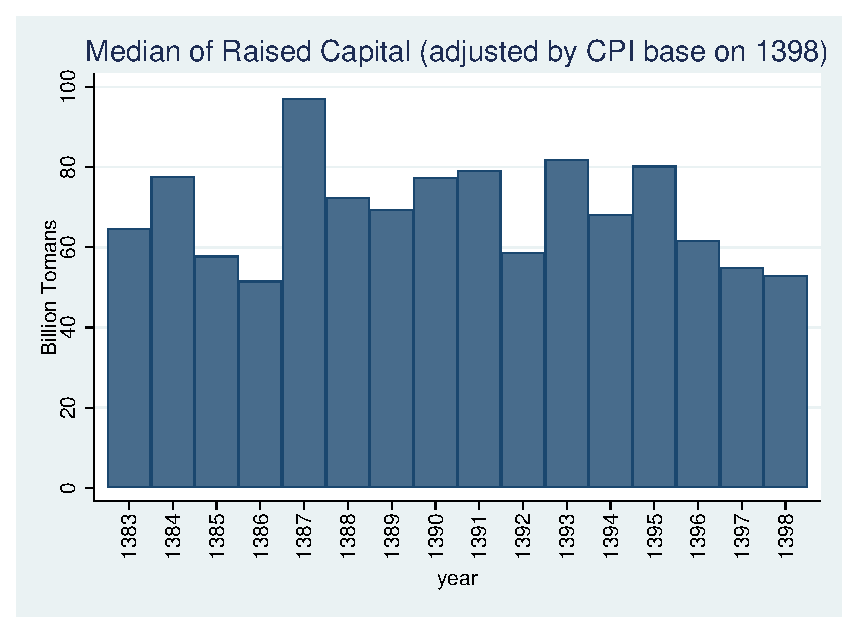
\includegraphics[width=0.7\linewidth]{MedianCapRaiseAdjusted.eps}
\label{fig:mediancapraise}
\end{figure}
\end{frame}

\begin{frame}{Data Summary}{Raised Capital for each Firm}
\begin{figure}
\centering
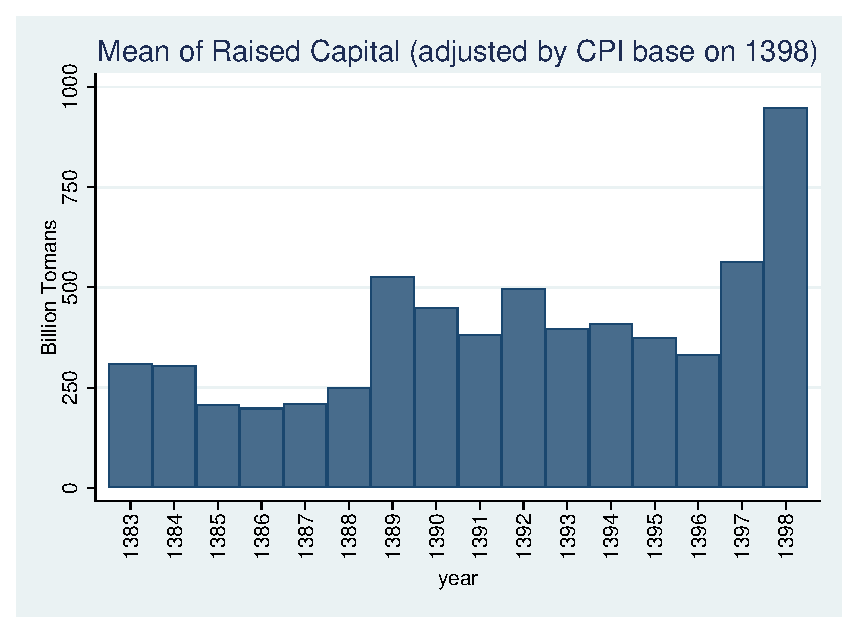
\includegraphics[width=0.7\linewidth]{MeanCapRaiseAdjusted.eps}
\label{fig:meancapraise}
\end{figure}
\end{frame}

\begin{frame}{Data Summary}{Adjusted Value of Raised Capital in market}
\begin{figure}
\centering
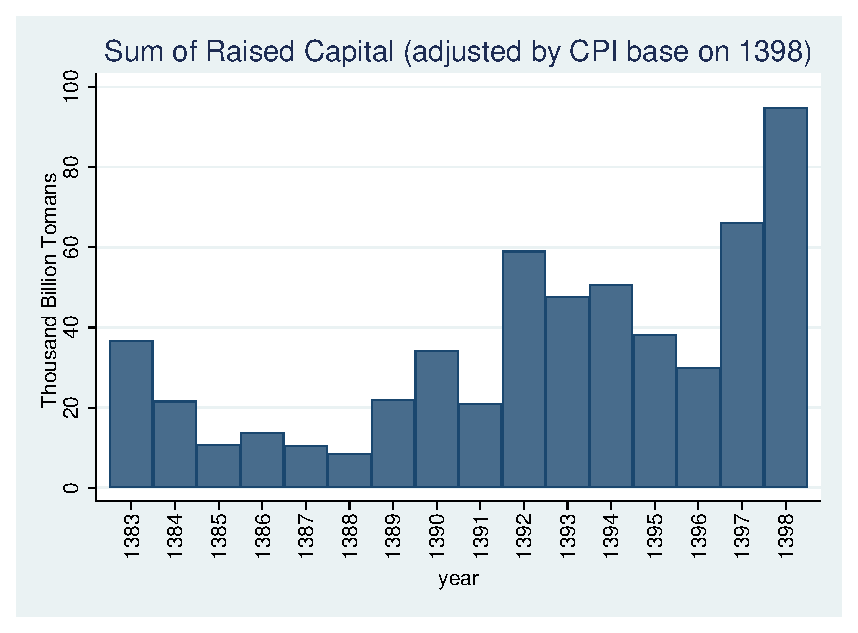
\includegraphics[width=0.7\linewidth]{SumCapRaiseAdjusted.eps}
\label{fig:SumCapRaise}
\end{figure}
\end{frame}



\begin{frame}{Data Summary}{Percent of Raised Capital for each Firm}
\begin{figure}
\centering
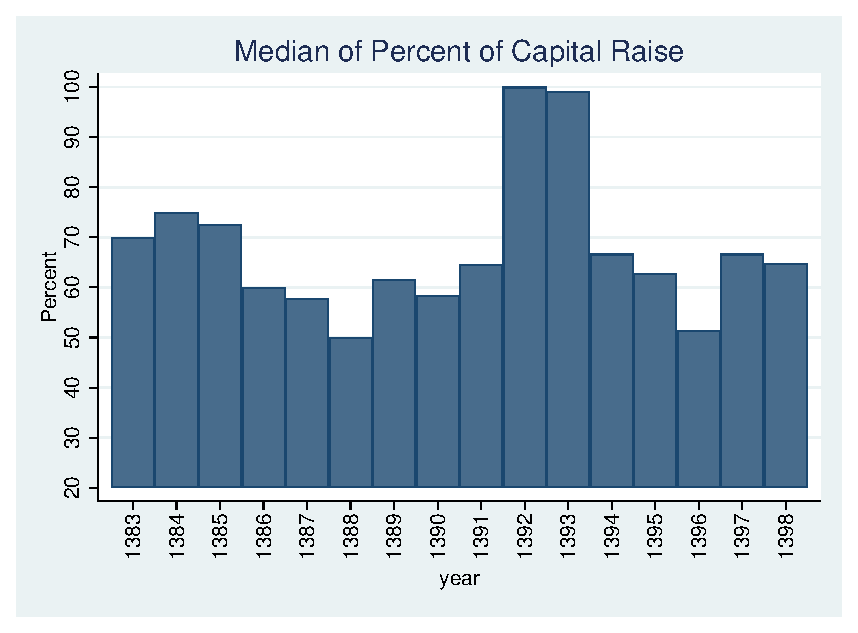
\includegraphics[width=0.7\linewidth]{MedianPercent.eps}
\label{fig:medianpercent}
\end{figure}
\end{frame}

\begin{frame}{Data Summary}{Number of Capital Raise}
\begin{figure}
\centering
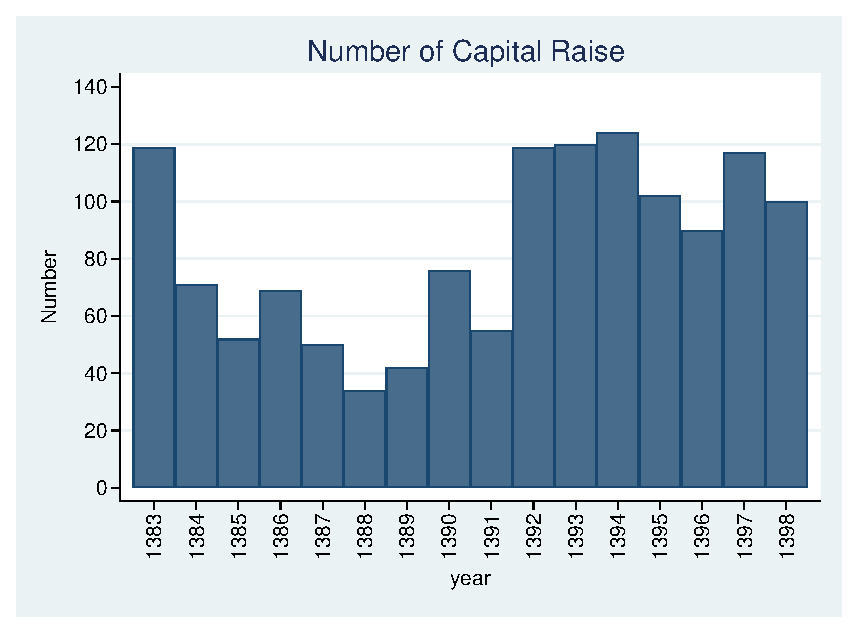
\includegraphics[width=0.7\linewidth]{Number.eps}
\label{fig:number}
\end{figure}
\end{frame}

\begin{frame}{Data Summary}{Number of Capital Raise}
\begin{figure}
\centering
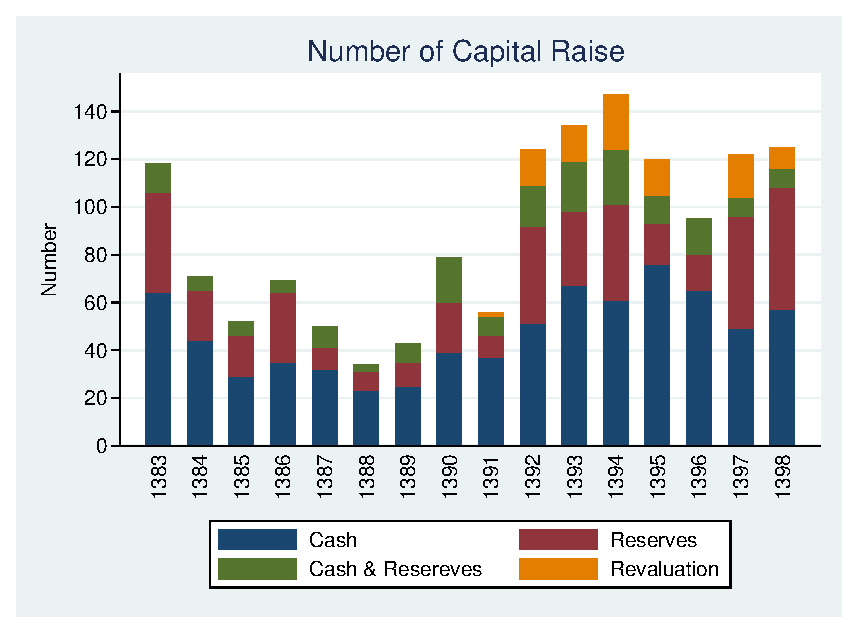
\includegraphics[width=0.7\linewidth]{Number2.eps}
\label{fig:number2}
\end{figure}

\end{frame}
%\begin{frame}{Number of Capital Raise}
%\begin{figure}
%\centering
%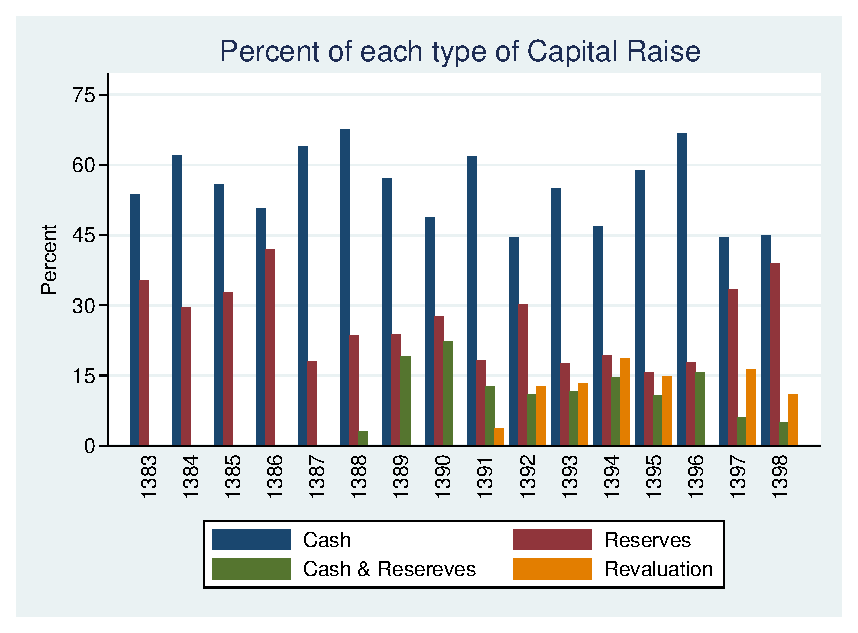
\includegraphics[width=0.7\linewidth]{Number3.eps}
%\label{fig:number3}
%\end{figure}
%\end{frame}

\begin{frame}{Number of Capital Raise for each Firm}
\begin{figure}
\centering
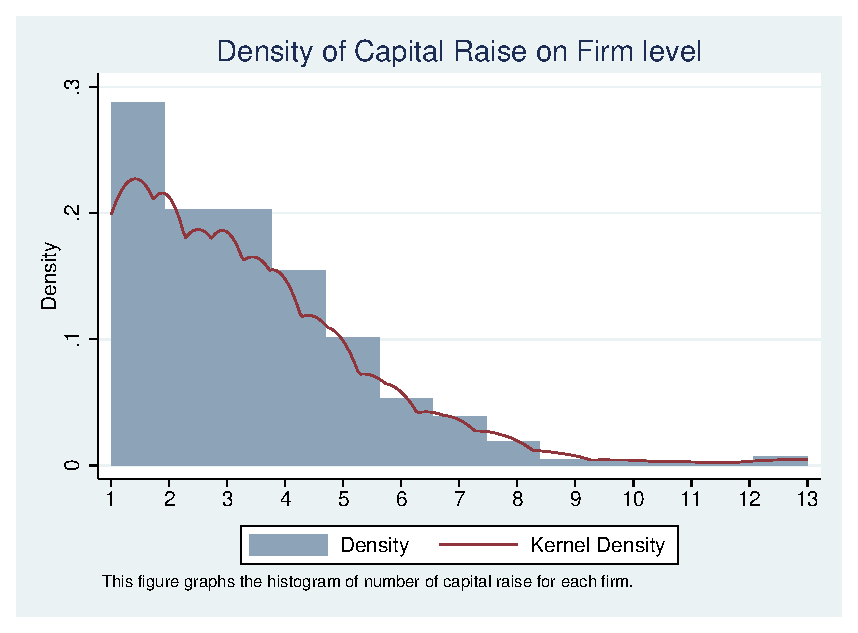
\includegraphics[width=0.7\linewidth]{Hist.eps}
\label{fig:Hist}
\end{figure}
\end{frame}

%\begin{frame}{Number of Capital Raise}
%\begin{figure}
%\centering
%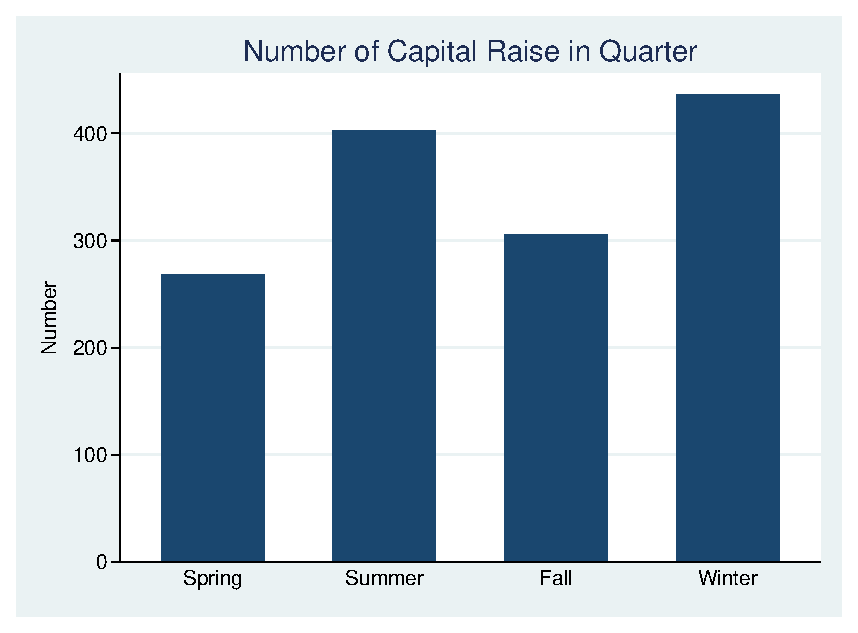
\includegraphics[width=0.7\linewidth]{QNumber}
%\label{fig:qnumber}
%\end{figure}
%\end{frame}
%
%\begin{frame}{Number of Capital Raise}
%\begin{figure}
%\centering
%\includegraphics[width=0.7\linewidth]{QNumber2}
%\label{fig:qnumber2}
%\end{figure}
%\end{frame}
%
%
%\begin{frame}{Number of Capital Raise}
%\begin{figure}
%\centering
%\includegraphics[width=0.7\linewidth]{QNumber3}
%\label{fig:qnumber3}
%\end{figure}
%\end{frame}
%
%
%
%
%
%
%
%\begin{frame}{Number of Capital Raise}
%\begin{figure}
%\centering
%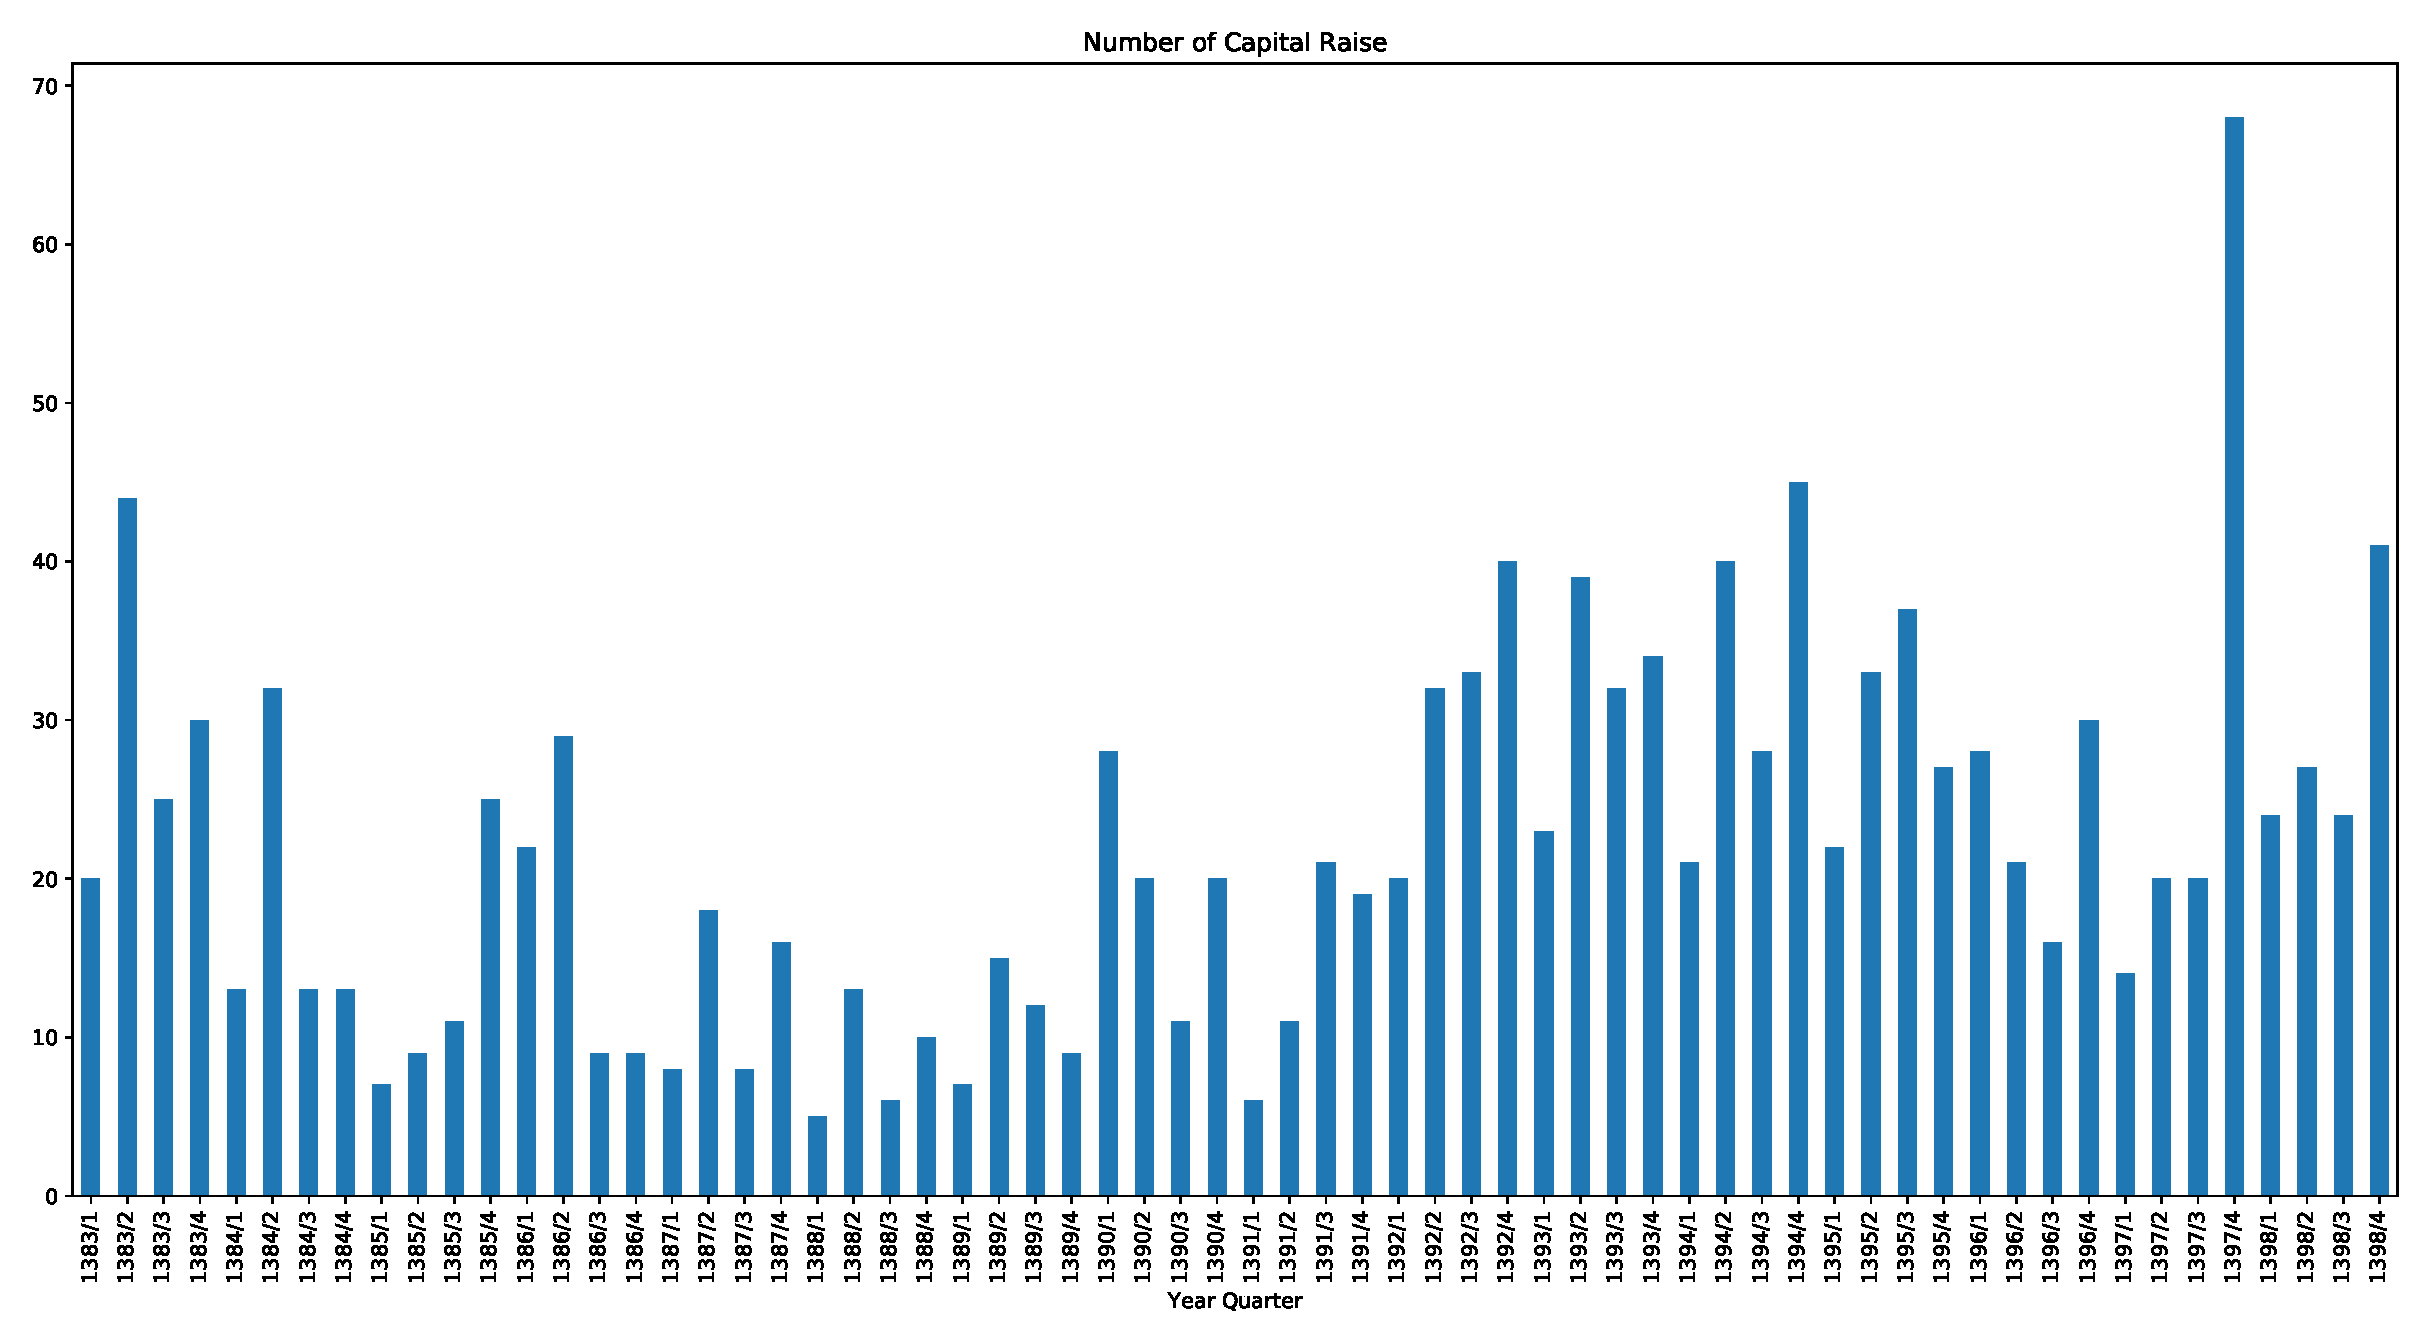
\includegraphics[width=1\linewidth]{Q2Number}
%\label{fig:q2number}
%\end{figure}
%\end{frame}
%
%\begin{frame}{Number of Capital Raise}
%\begin{figure}
%\centering
%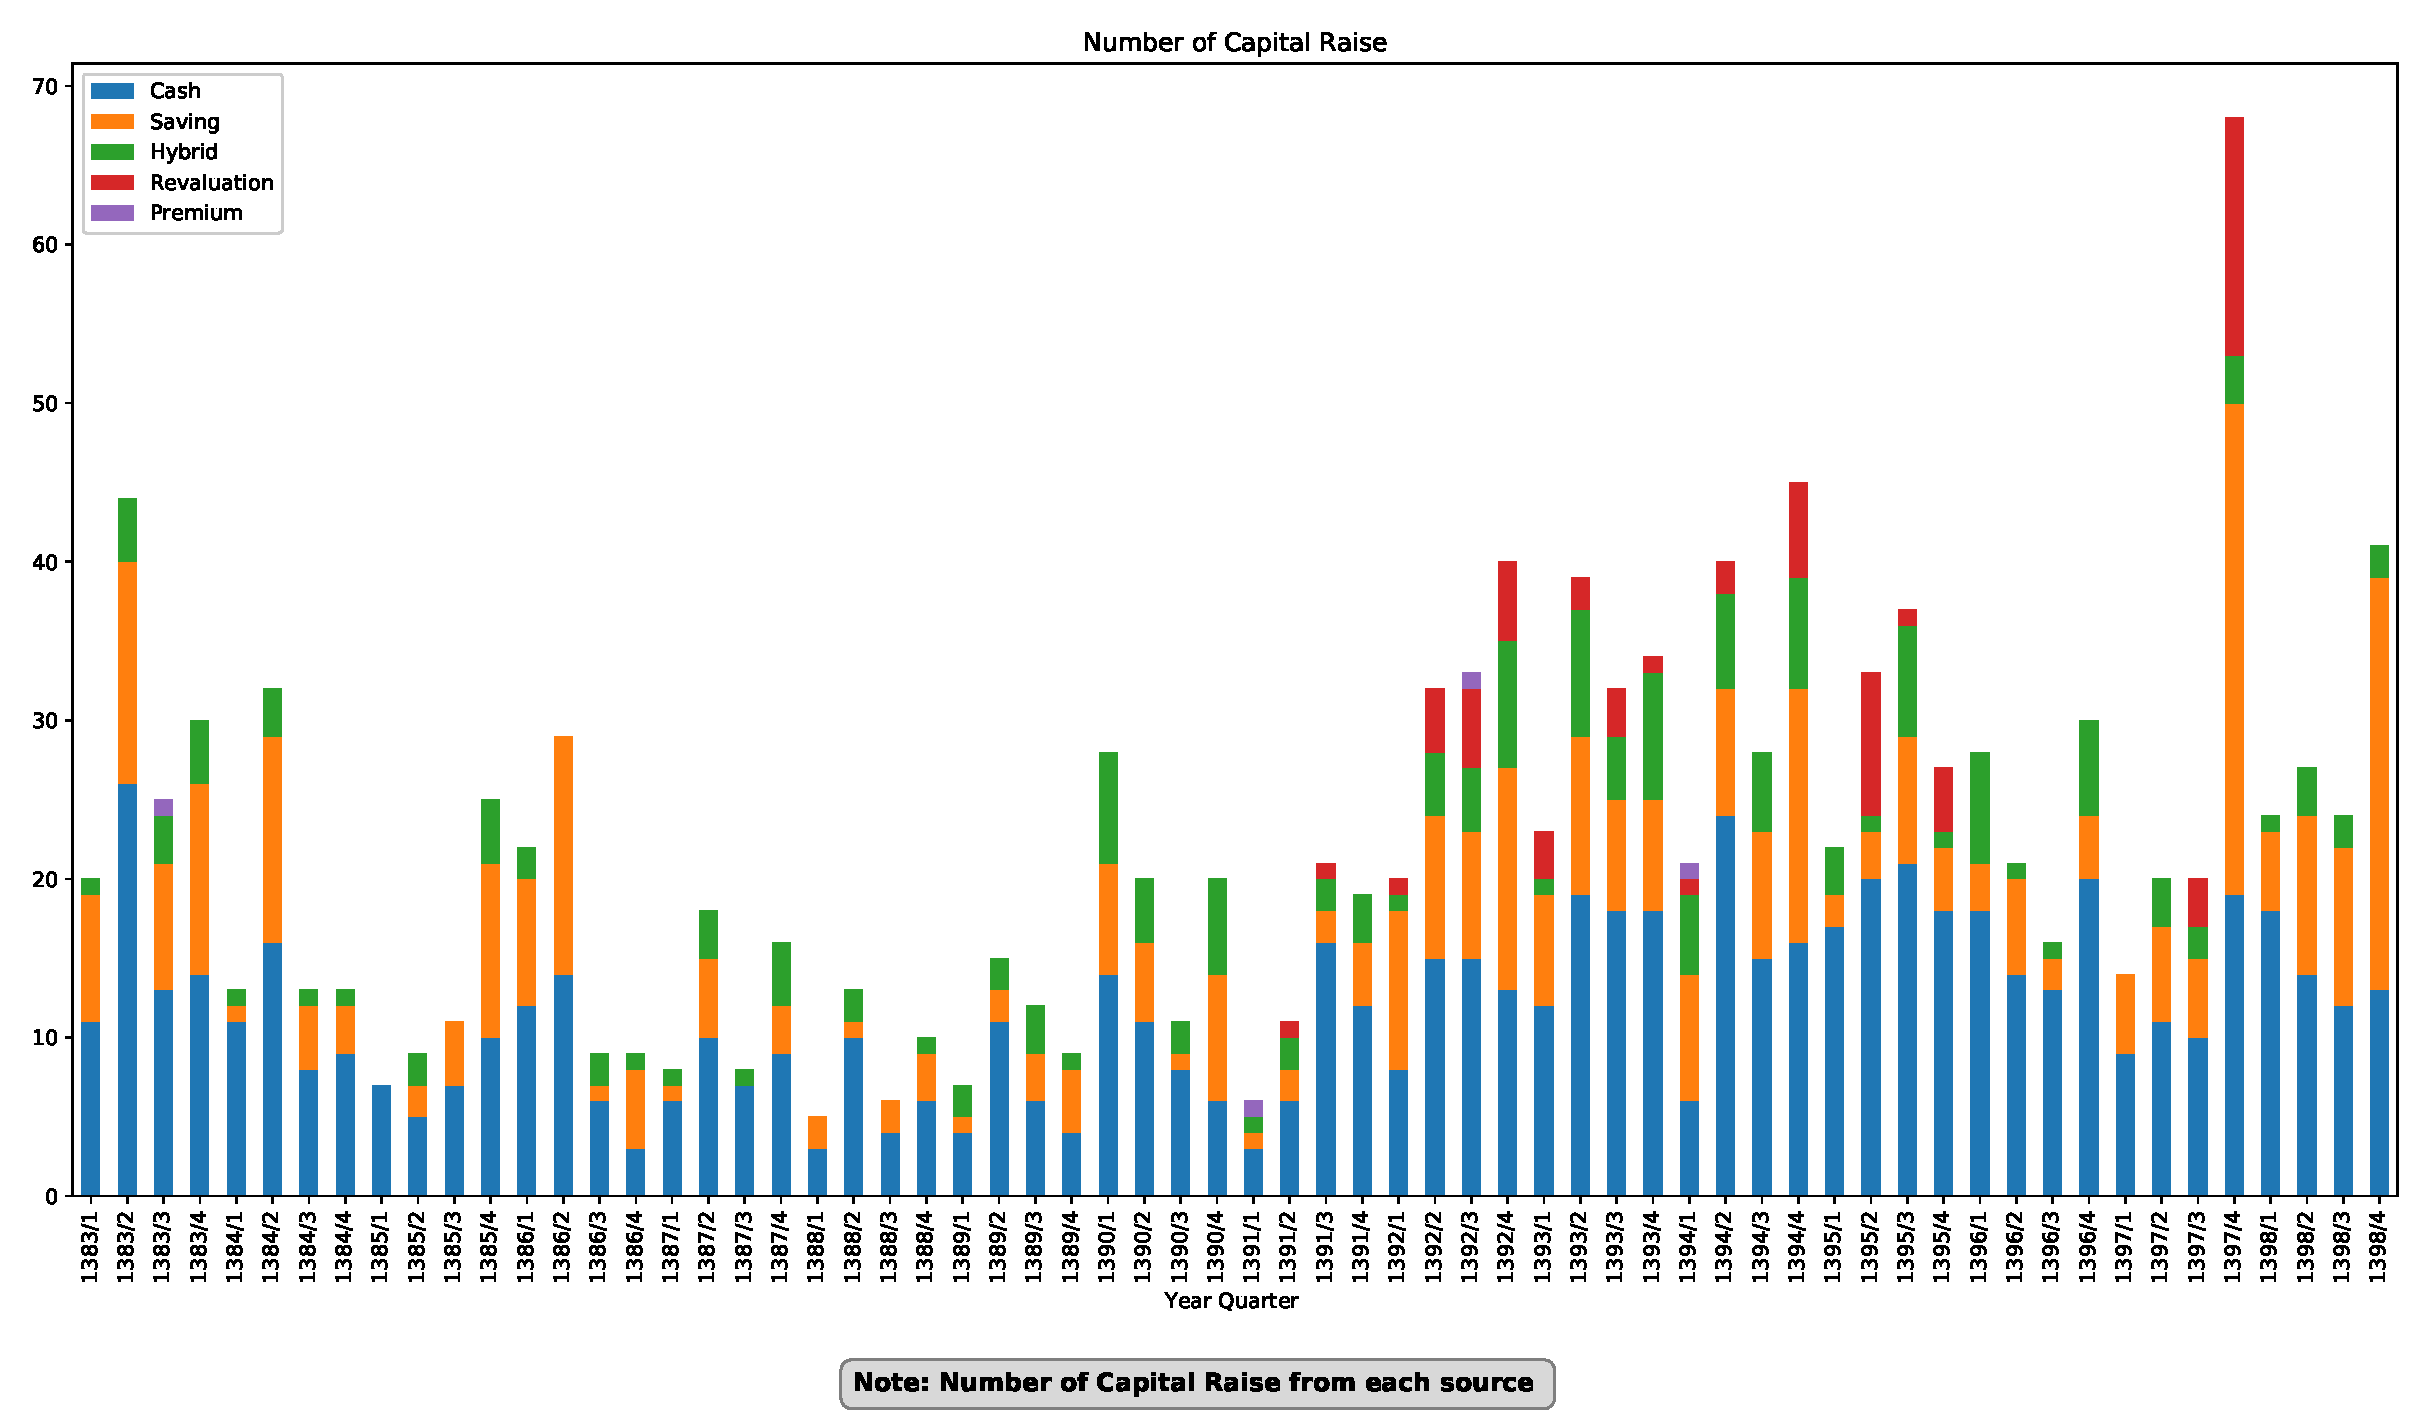
\includegraphics[width=1\linewidth]{Q2Number2}
%\label{fig:q2number2}
%\end{figure}
%\end{frame}


\section{Abnormal Return}

\begin{frame}{Abnormal Return}
\begin{itemize}
\item Abnormal return  is the difference between the observed return and the predicted return
\begin{equation*}
AR_{i,t} = R_{i,t} - E(R_{i,t}|X_t)
\end{equation*}
\item Predicted return
\begin{itemize}
\item Mean-adjusted returns Model (MAR) $ \longrightarrow \bar{R}_i $
\item Market-adjusted returns Model (MKAR) $ \longrightarrow {R}_{M,t} $
\item Risk-adjusted returns Model (RAR) $ \longrightarrow \alpha_i + \beta_i{R}_{M,t} $
\end{itemize}
\end{itemize}
\end{frame}
\begin{frame}{Abnormal Return Calculation}{First Step}


%\item  Fama, Fisher, Jensen and Roll (1969)
%
%\begin{tikzpicture}
%	\draw[] (0,0) -- node[below=1mm,pos=0.6,scale=2]{}(10,0)node[right = 4mm]{};
%	\draw[] (1,2.5mm)-- +(0,-5.5mm)node[below]{$T_0$};	
%	\draw[] (5,2.5mm) -- +(0,-5.5mm)node[below]{$0$};
%	\draw[] (9,2.5mm) -- +(0,-5.5mm)node[below]{$T_1$};
%	
%\draw [decorate,decoration={brace,amplitude=5pt,,raise=2ex}]
%  (1,0) -- (9,0) node[midway,yshift=2em]{Estimation Window \& Event Window};
%
%	\end{tikzpicture}





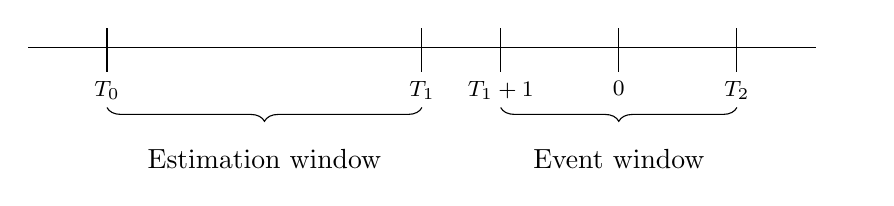
\begin{tikzpicture}
	\draw[] (0,0) -- node[below=1mm,pos=0.6,scale=2]{}(10,0)node[right = 4mm]{};
	\draw[] (1,2.5mm) -- +(0,-5.5mm)node[below]{\footnotesize $T_0$};	
	\draw[] (5,2.5mm) -- +(0,-5.5mm)node[below]{\footnotesize$T_1$};
	\draw[] (6,2.5mm) -- +(0,-5.5mm)node[below]{\footnotesize$T_1 + 1$};
	\draw[] (9,2.5mm)  -- +(0,-5.5mm)node[below]{\footnotesize$T_2$};
	\draw[] (7.5,2.5mm) -- +(0,-5.5mm)node[below]{\footnotesize $0$};
	
\draw [decorate,decoration={brace,amplitude=5pt,mirror,raise=5ex}]
  (1,0) -- (5,0) node[midway,yshift=-4em]{Estimation window};
  \draw [decorate,decoration={brace,amplitude=5pt,mirror,raise=5ex}]
    (6,0) -- (9,0) node[midway,yshift=-4em]{Event window};
	\end{tikzpicture}
\begin{itemize}
\item Event windows specifically 3-day, 7-day, and 11-day event periods 
\item  Estimation window :  Each event window implies a particular estimation window interval.
\scriptsize(For example,
3-day event window [-1,+1] is associated with [-122,-2] estimation window)
\normalsize
\item Fama,Fisher,Jensen, and Roll use Event Window as Estimation window  
\tiny[IER-1969-The Adjustment of Stock Prices to New Information]
\end{itemize}
\end{frame}


\begin{frame}{Abnormal Return Calculation}{Second Step}
\begin{itemize}
\scriptsize
\item For each Firm :
\begin{equation*}
R_{i,t} = \hat{\alpha}_i + \hat{\beta}_i (R_{m,t}) + \boxed{\varepsilon_{i,t}} \rightarrow AR_{i,t}
\end{equation*}

\item Average abnormal return during period t: 
\tiny $ N_t $ is the number of firms in the sample during period t
\scriptsize
\begin{equation*}
AAR_t = \sum_{i=1}^{N_t} \frac{AR_{it}}{N_t}
\end{equation*}
\item Cumulative Abnormal Returns
\begin{equation*}
CAR_t(t_1,t_2) = \sum_{t=t_1}^{t_2} {AR_{it}}
\end{equation*}
\item Cumulative Average Abnormal Return from period $ t_1 $ to period $ t_2 $
\begin{equation*}
CAAR_{t_1,t_2} = \sum_{i=t_1}^{t_2} CAR_i(t_1,t_2)
\end{equation*}
\end{itemize}
\end{frame}


\begin{frame}{Abnormal Return Calculation}{Cross-Sectional Test (Test $ AAR=0 $)}


 \begin{itemize}
\item Hypothesis is  $\left\{\begin{array}{c c }
H_0: & AAR=0\\
H_1: & AAR\neq 0
\end{array}\right.
$\\
\item[]
\item The t-statistics for this test is 
\begin{itemize}
\item 
$
t_{AAR} = \sqrt{N}\frac{AAR}{S_{AAR}}
$
\item 
$
S^2_{AAR} = \frac{1}{N-1}\sum_{i = 1}^{N}(AR_i - {AAR})^2
$
\end{itemize}
\end{itemize}



\end{frame}


\begin{frame}{Abnormal Return Calculation}{Cross-Sectional Test (Test $ CAAR=0 $ )}
     
 \begin{itemize}
\item Hypothesis is  $\left\{\begin{array}{c c }
H_0: & CAAR=0\\
H_1: & CAAR\neq 0
\end{array}\right.
$\\
\item[]
\item The t-statistics for this test is 
\begin{itemize}
\item 
$
t_{CAAR} = \sqrt{N}\frac{CAAR}{S_{CAAR}}
$
\item 
$
S^2_{CAAR} = \frac{1}{N-1}\sum_{i = 1}^{N}(CAR_i - {CAAR})^2
$
\item
\scriptsize
 $ CAR_i = \sum_{i=t_1}^{t_2} AR_{i,t} $ 
\normalsize 
\end{itemize}
\end{itemize}

\end{frame}



\section{Literature}

\begin{frame}
	\scriptsize
	\begin{itemize}
		\item Price reaction to equity issue announcements in high equity issue volume (HOT) periods is lower on average than in low equity issue volume (COLD) periods. [\cite{bayless1996there}]
		
		\item Firms significantly under perform all of benchmarks
		over the five years following the equity issues. 
		[\cite{jegadeesh2000long}]
		\begin{itemize}
			\tiny
			\item Similar levels of under performance for both small firms and large firms, and both growth firms and value
			firms. 
			\item Factor-model benchmarks are miss specified
		\end{itemize}
	\item  Under performance is concentrated primarily in small issuing
	firms with low book to market ratios. [\cite{brav2000abnormal}]
	\item Price reaction to right issues for listed Indian firms is a positive but statistically insignificant.[\cite{marisetty2008price}]
	\begin{itemize}
		\tiny
		\item The price reaction is significantly more negative for firms with a family group affiliation
		compared to firms with no family group affiliation
	\end{itemize}
	\item When shareholders approve issuances, average announcement returns are positive \tiny[\cite{holderness2018equity}]
	\begin{itemize}
		\tiny
		\item  Agency problems affect equity issuances and challenge existing adverse selection, market timing, and
		signaling explanations.
	\end{itemize}
	\end{itemize}
	
\end{frame}
\normalsize
\begin{frame}{Iran}
\begin{figure}
\centering
\includegraphics[width=0.65\linewidth]{Soltani}
\label{Soltani}
\end{figure}
\end{frame}


\section{Abnormal Return Results}
\begin{frame}{Abnormal Return}


\begin{itemize}
\item We use the Risk-adjusted returns Model (CAPM) to predict returns.
\begin{itemize}
\item We accumulate factors' return in close days for using in the model.
\end{itemize}
\item We set estimation and event window as:\\
\begin{figure}[htbp]
\centering
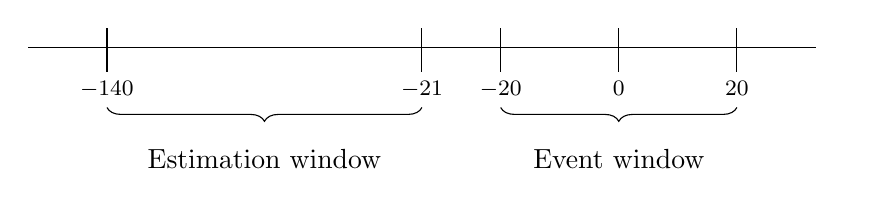
\begin{tikzpicture}
	\draw[] (0,0) -- node[below=1mm,pos=0.6,scale=2]{}(10,0)node[right = 4mm]{};
	\draw[] (1,2.5mm) -- +(0,-5.5mm)node[below]{\footnotesize $-140$};	
	\draw[] (5,2.5mm) -- +(0,-5.5mm)node[below]{\footnotesize$-21$};
	\draw[] (6,2.5mm) -- +(0,-5.5mm)node[below]{\footnotesize$-20$};
	\draw[] (9,2.5mm)  -- +(0,-5.5mm)node[below]{\footnotesize$20$};
	\draw[] (7.5,2.5mm) -- +(0,-5.5mm)node[below]{\footnotesize $0$};
	
\draw [decorate,decoration={brace,amplitude=5pt,mirror,raise=5ex}]
  (1,0) -- (5,0) node[midway,yshift=-4em]{Estimation window};
  \draw [decorate,decoration={brace,amplitude=5pt,mirror,raise=5ex}]
    (6,0) -- (9,0) node[midway,yshift=-4em]{Event window};
	\end{tikzpicture}

\end{figure}

\item We test whether $ CAAR=0 $ or not
\end{itemize}
\end{frame}

\begin{frame}{Estimation Results}
\begin{table}[htbp]
\resizebox{0.7\textwidth}{!}{
    \begin{tabular}{lccccccc}
    \hline\hline
          & mean  & std   & min   & 25\%  & 50\%  & 75\%  & max \\
          \hline
    Beta CAPM & 0.80  & 0.84  & -3.62 & 0.28  & 0.69  & 1.18  & 8.81 \\
    Alpha CAPM & 0.16  & 0.39  & -2.42 & -0.05 & 0.09  & 0.28  & 3.60 \\
    \hline
    Beta Market & 0.79  & 0.73  & -5.41 & 0.32  & 0.72  & 1.19  & 4.65 \\
    Beta SMB & 0.14  & 0.28  & -1.14 & -0.01 & 0.07  & 0.22  & 2.33 \\
    Beta HML & 0.02  & 0.27  & -1.43 & -0.09 & 0.02  & 0.14  & 1.65 \\
    Beta WL & 0.06  & 0.26  & -0.71 & -0.07 & 0.03  & 0.15  & 2.10 \\
    Alpha Four & 0.10  & 0.41  & -2.15 & -0.07 & 0.06  & 0.22  & 4.71 \\
    \hline\hline
    \end{tabular}%
}
\end{table}
\end{frame}

\subsection{Abnormal Return}
\begin{frame}{Abnormal Return}
\label{abreturn}
\begin{figure}
\centering
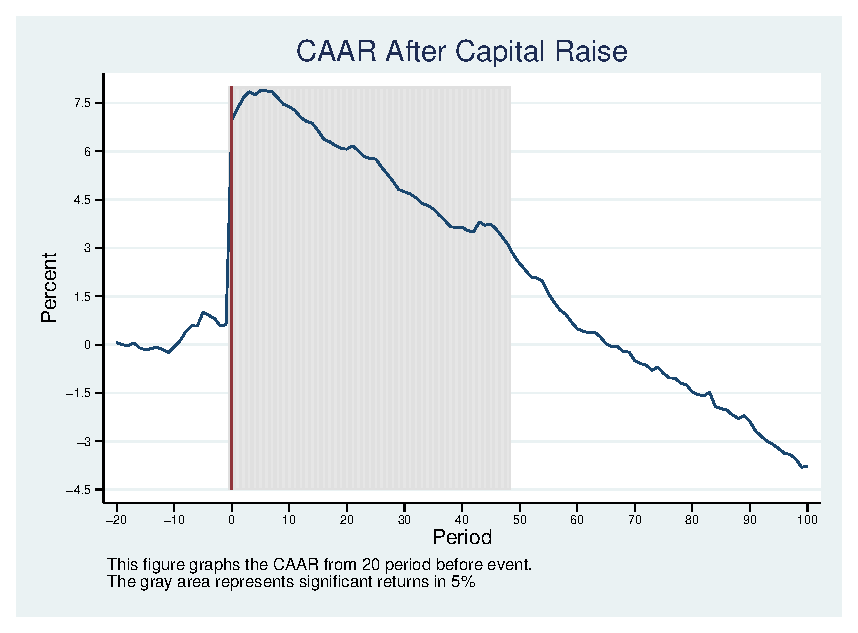
\includegraphics[width=0.7\linewidth]{AbReturn.eps}
\label{fig:abreturn}
\end{figure}

\hfill\hyperlink{abreturn4Factor}{\beamerbutton{4Factor}}

\end{frame}

\begin{frame}
% Table generated by Excel2LaTeX from sheet 'Sheet1'


 \centering
\begin{table}[htbp]
  \centering
  
\captionsetup{labelformat=empty}
  \caption{\tiny Analysis of abnormal return in days surrounding the capital raise announcements}
  \centering
  \resizebox{0.8\textheight}{!}
  {\tiny
    \begin{tabular}{cccc|cccc}
    \hline\hline
    Period & \multicolumn{1}{c}{AAR} & \multicolumn{1}{c}{CAAR} & \multicolumn{1}{c}{t-stat} & Period & \multicolumn{1}{c}{AAR} & \multicolumn{1}{c}{CAAR} & \multicolumn{1}{c}{t-stat} \\
    \hline    -20   & 0.06  & 0.06  & 0.45  & 0     & 6.38  & 6.99  & 7.88 \\
        -19   & -0.06 & 0.00  & -0.02 & 1     & 0.33  & 7.32  & 8.10 \\
        -18   & -0.03 & -0.03 & -0.15 & 2     & 0.32  & 7.67  & 8.34 \\
        -17   & 0.08  & 0.05  & 0.23  & 3     & 0.18  & 7.85  & 8.39 \\
        -16   & -0.16 & -0.10 & -0.42 & 4     & -0.07 & 7.75  & 8.12 \\
        -15   & -0.06 & -0.16 & -0.59 & 5     & 0.13  & 7.89  & 7.95 \\
        -14   & 0.04  & -0.13 & -0.43 & 6     & -0.02 & 7.88  & 7.87 \\
        -13   & 0.05  & -0.08 & -0.24 & 7     & -0.08 & 7.85  & 7.77 \\
        -12   & -0.08 & -0.16 & -0.47 & 8     & -0.19 & 7.65  & 7.52 \\
        -11   & -0.09 & -0.25 & -0.68 & 9     & -0.22 & 7.46  & 7.24 \\
        -10   & 0.18  & -0.06 & -0.17 & 10    & -0.07 & 7.39  & 7.08 \\
        -9    & 0.18  & 0.12  & 0.29  & 11    & -0.12 & 7.27  & 6.88 \\
        -8    & 0.29  & 0.40  & 0.93  & 12    & -0.22 & 7.05  & 6.65 \\
        -7    & 0.16  & 0.59  & 1.30  & 13    & -0.11 & 6.93  & 6.46 \\
        -6    & -0.01 & 0.58  & 1.23  & 14    & -0.04 & 6.87  & 6.28 \\
        -5    & 0.41  & 1.00  & 1.80  & 15    & -0.19 & 6.64  & 6.02 \\
        -4    & -0.09 & 0.91  & 1.59  & 16    & -0.26 & 6.38  & 5.71 \\
        -3    & -0.11 & 0.81  & 1.37  & 17    & -0.10 & 6.30  & 5.54 \\
        -2    & -0.22 & 0.58  & 0.95  & 18    & -0.15 & 6.18  & 5.36 \\
        -1    & 0.04  & 0.62  & 1.01  & 19    & -0.09 & 6.09  & 5.24 \\
    \hline\hline
    \end{tabular}%
}
\end{table}%

\end{frame}
%
%\begin{frame}{Abnormal Return}
%\begin{figure}
%\centering
%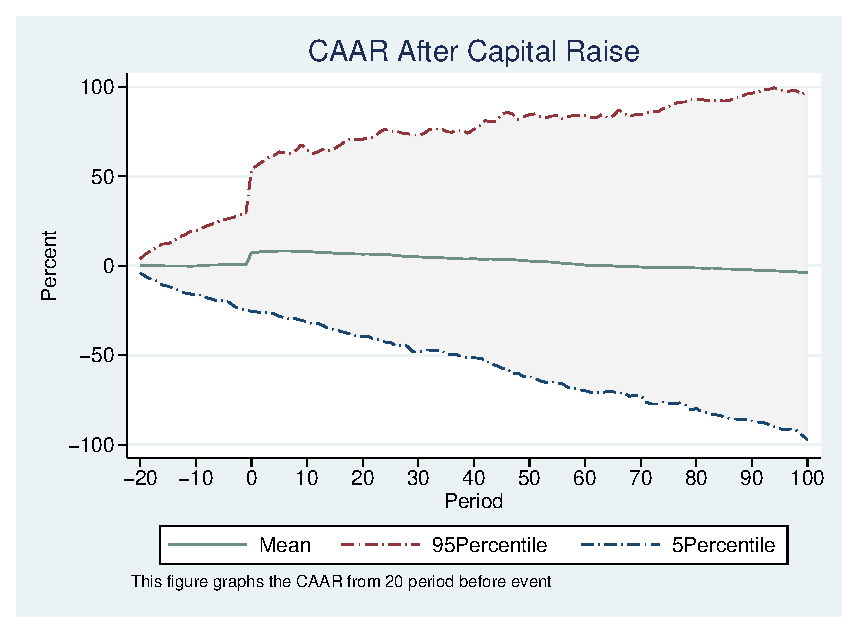
\includegraphics[width=0.7\linewidth]{95-5AbReturn.eps}
%\label{fig:95-5AbReturn}
%\end{figure}
%\end{frame}





\begin{frame}{Abnormal Return}{Abnormal return of raised capital from Revaluation}
\label{abreturnrevalution}
\begin{figure}
\centering
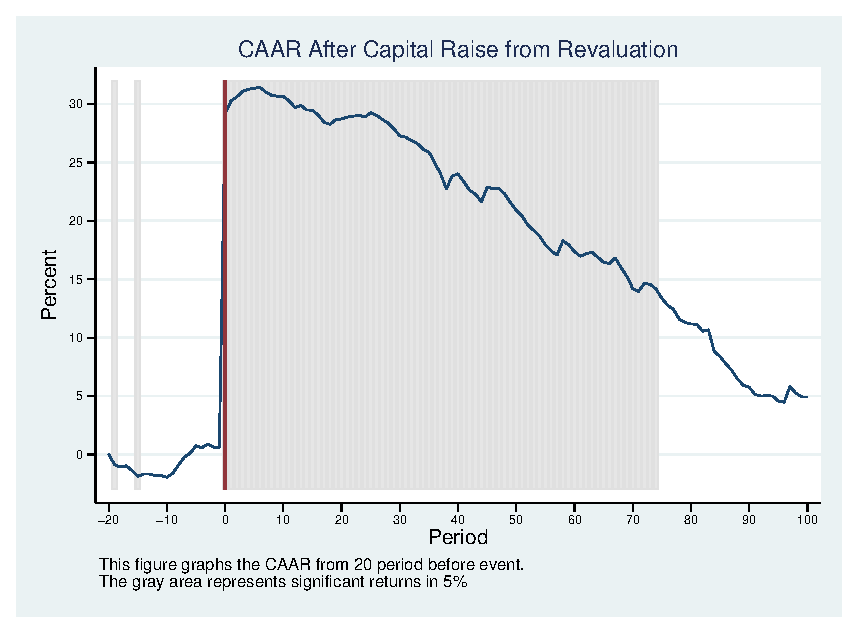
\includegraphics[width=0.65\linewidth]{AbReturnRevalution}
\label{fig:abreturnrevalution}
\end{figure}

\hfill\hyperlink{abreturnrevalution4Factor}{\beamerbutton{4Factor}}
\end{frame}


\begin{frame}

 \centering
\begin{table}[htbp]
  \centering
  
\captionsetup{labelformat=empty}
  \caption{\tiny Analysis of abnormal return in days surrounding the Revaluation announcements}
  \resizebox{0.8\textheight}{!}
  {\tiny
    \begin{tabular}{cccc|cccc}
    \hline\hline 
      Period & \multicolumn{1}{c}{AAR} & \multicolumn{1}{c}{CAAR} & \multicolumn{1}{c}{t-stat} & Period & \multicolumn{1}{c}{AAR} & \multicolumn{1}{c}{CAAR} & \multicolumn{1}{c}{t-stat} \\
      \hline
        -20   & 0.04  & 0.04  & 0.13  & 0     & 28.55 & 29.18 & 6.41 \\
        -19   & -0.89 & -0.86 & -2.02 & 1     & 1.08  & 30.26 & 6.58 \\
        -18   & -0.26 & -1.08 & -1.83 & 2     & 0.35  & 30.61 & 6.58 \\
        -17   & 0.11  & -0.97 & -1.50 & 3     & 0.47  & 31.08 & 6.55 \\
        -16   & -0.39 & -1.36 & -1.82 & 4     & 0.17  & 31.25 & 6.43 \\
        -15   & -0.52 & -1.88 & -2.26 & 5     & 0.10  & 31.36 & 6.34 \\
        -14   & 0.21  & -1.67 & -1.72 & 6     & 0.07  & 31.42 & 6.26 \\
        -13   & 0.00  & -1.67 & -1.48 & 7     & -0.40 & 31.02 & 6.11 \\
        -12   & -0.14 & -1.81 & -1.40 & 8     & -0.28 & 30.74 & 6.01 \\
        -11   & 0.02  & -1.80 & -1.35 & 9     & -0.07 & 30.67 & 5.90 \\
        -10   & -0.15 & -1.95 & -1.45 & 10    & -0.02 & 30.65 & 5.83 \\
        -9    & 0.33  & -1.61 & -1.15 & 11    & -0.38 & 30.27 & 5.66 \\
        -8    & 0.72  & -0.89 & -0.59 & 12    & -0.59 & 29.68 & 5.59 \\
        -7    & 0.67  & -0.22 & -0.14 & 13    & 0.21  & 29.89 & 5.62 \\
        -6    & 0.33  & 0.12  & 0.07  & 14    & -0.15 & 29.49 & 5.39 \\
        -5    & 0.63  & 0.75  & 0.44  & 15    & -0.02 & 29.47 & 5.34 \\
        -4    & -0.16 & 0.58  & 0.32  & 16    & -0.43 & 29.05 & 5.21 \\
        -3    & 0.30  & 0.89  & 0.43  & 17    & -0.61 & 28.43 & 5.09 \\
        -2    & -0.26 & 0.63  & 0.29  & 18    & -0.17 & 28.27 & 5.02 \\
        -1    & 0.01  & 0.63  & 0.28  & 19    & 0.39  & 28.65 & 5.03 \\
    \hline\hline
    \end{tabular}%
}
\end{table}%

    
\end{frame}



\begin{frame}{Abnormal Return}{Abnormal return of raised capital from Reserves}
\label{abreturnsaving}
\begin{figure}
\centering
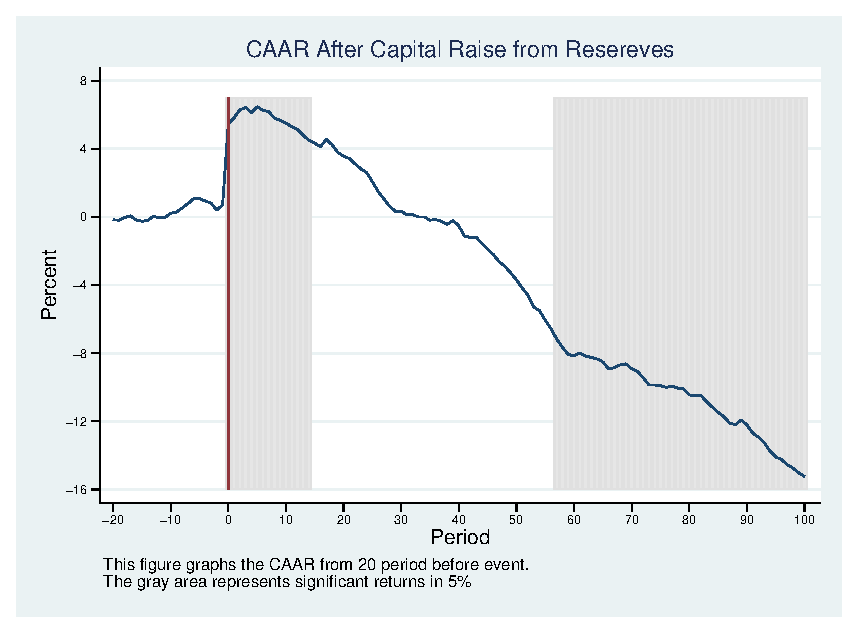
\includegraphics[width=0.65\linewidth]{AbReturnSaving}
\label{fig:abreturnsaving}
\end{figure}

\hfill\hyperlink{abreturnsaving4Factor}{\beamerbutton{4Factor}}
\end{frame}




\begin{frame}{Abnormal Return}{Abnormal return of raised capital from Cash}
\label{abreturncash}
\begin{figure}
\centering
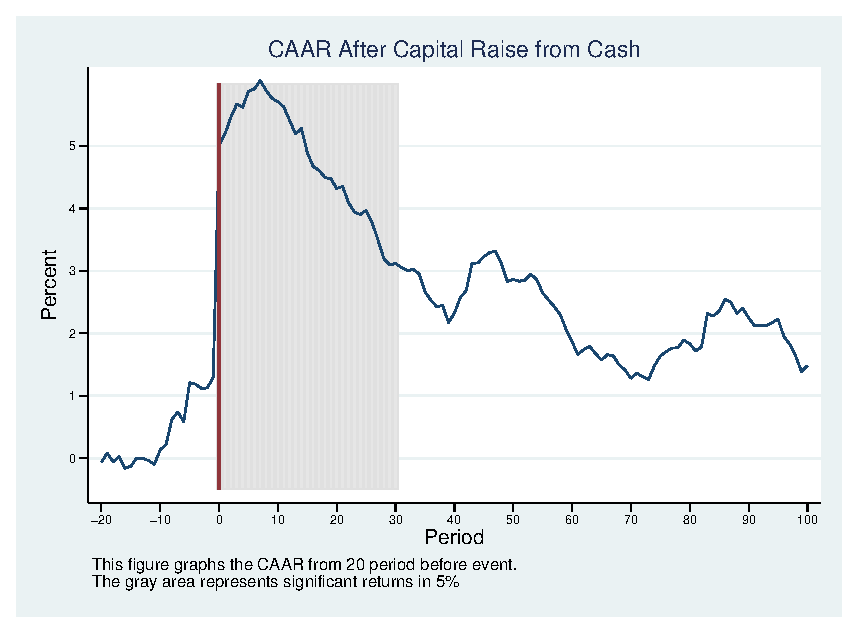
\includegraphics[width=0.65\linewidth]{AbReturnCash}
\label{fig:abreturncash}
\end{figure}
\hfill\hyperlink{abreturncash4Factor}{\beamerbutton{4Factor}}
\end{frame}





\begin{frame}{Abnormal Return}{Abnormal return of raised capital from Cash \& Reserves}
\label{abreturnhybrid}
\begin{figure}
\centering
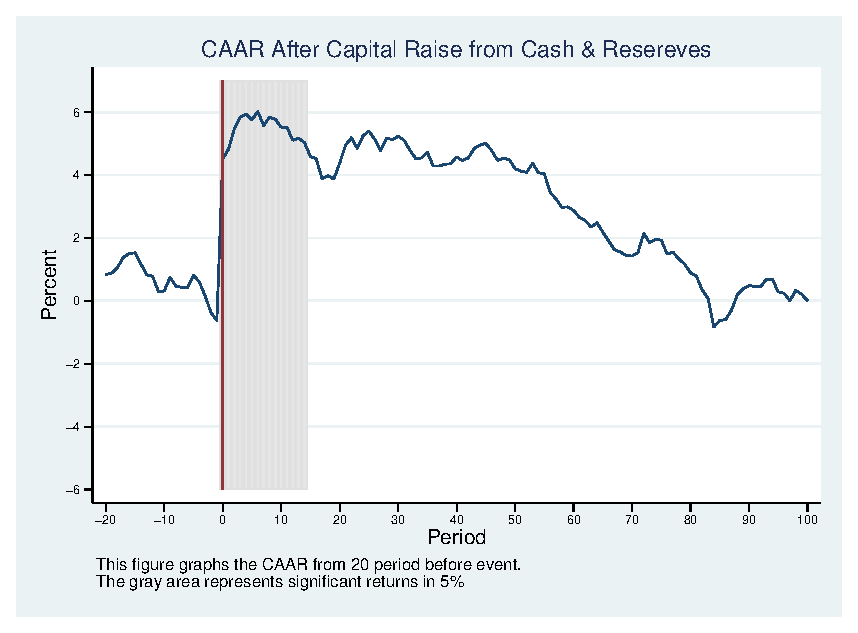
\includegraphics[width=0.65\linewidth]{AbReturnHybrid}
\label{fig:abreturnhybrid}
\end{figure}
\hfill\hyperlink{abreturnhybrid4Factor}{\beamerbutton{4Factor}}
\end{frame}


\begin{frame}
\label{AbReturn_year}
\begin{figure}
\centering
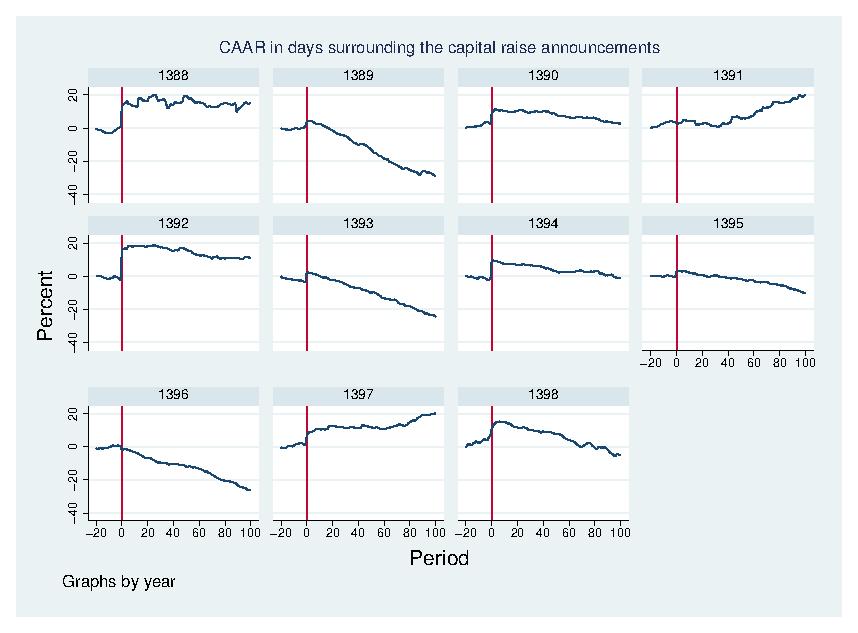
\includegraphics[width=0.85\linewidth]{AbReturn_year.eps}
\label{fig:AbReturn_year}
\end{figure}


\end{frame}


\begin{frame}
\label{AbReturn_year_Revaluation}
\begin{figure}
\centering
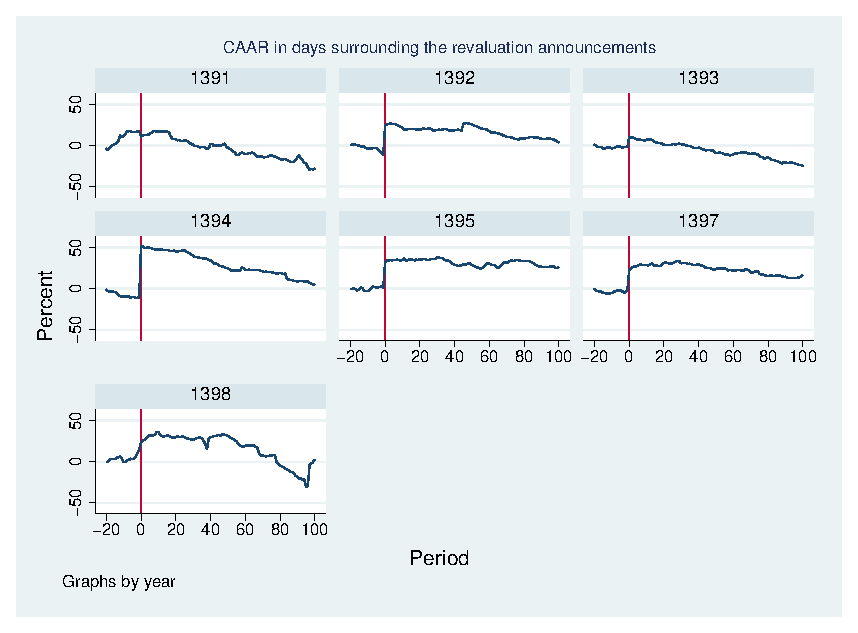
\includegraphics[width=0.85\linewidth]{AbReturn_year_Revaluation.eps}
\label{fig:AbReturn_year_Revaluation}
\end{figure}


\end{frame}

\begin{frame}
\label{AbReturn_year_NoRevaluation}
\begin{figure}
\centering
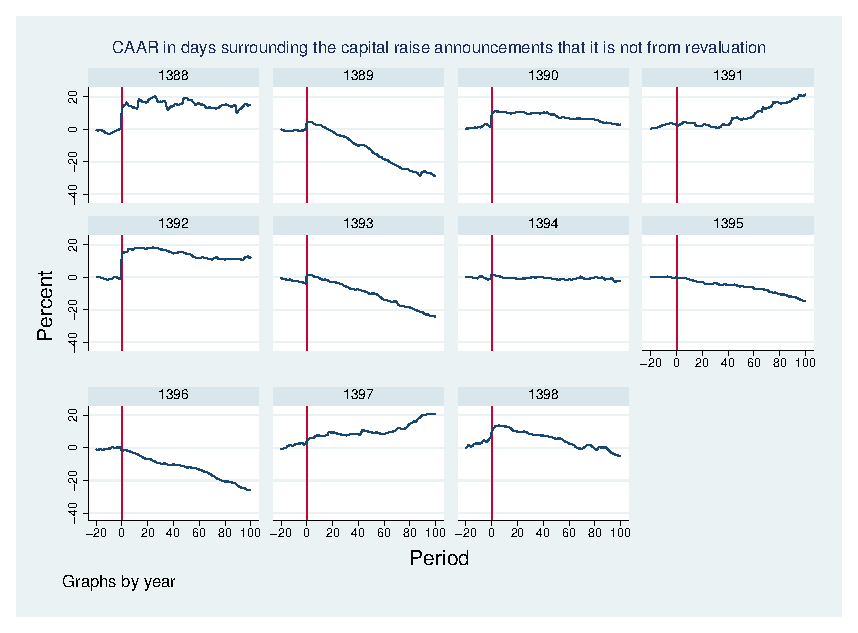
\includegraphics[width=0.85\linewidth]{AbReturn_year_NoRevaluation.eps}
\label{fig:AbReturn_year_NoRevaluation}
\end{figure}


\end{frame}

\subsection{Volume}

\begin{frame}{Volume}
\begin{figure}
\centering
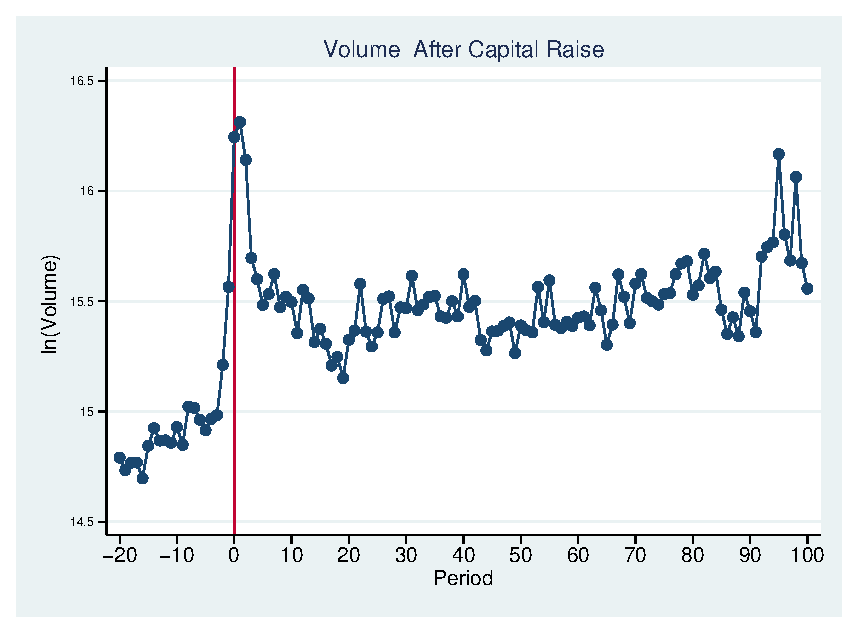
\includegraphics[width=0.7\linewidth]{volume}
\label{fig:volume}
\end{figure}
\end{frame}


\begin{frame}{Volume}{Volume of raised capital from Revaluation}
\begin{figure}
\centering
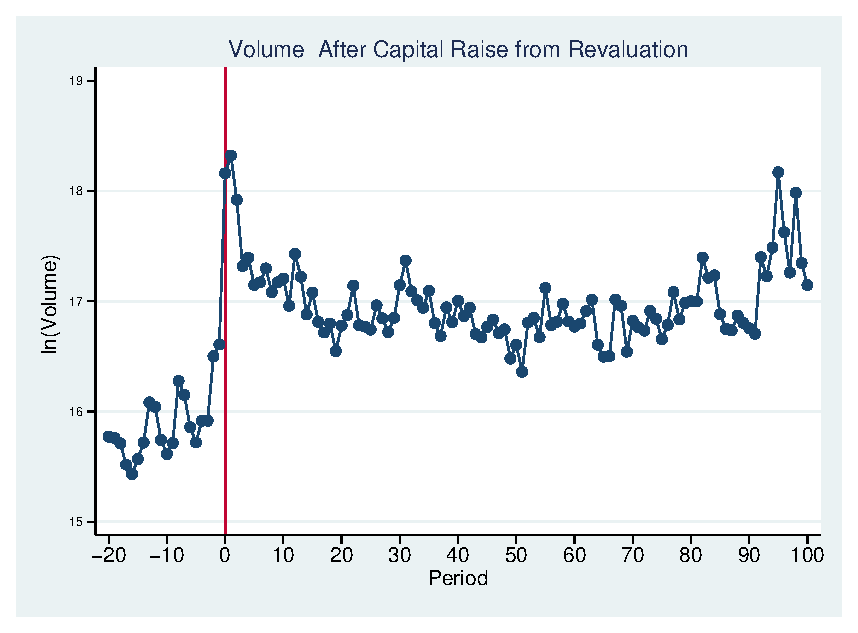
\includegraphics[width=0.7\linewidth]{volume_Revaluation}
\label{fig:volumerevaluation}
\end{figure}
\end{frame}


\begin{frame}{Volume}{Volume of raised capital that it's not from Revaluation}
\begin{figure}
\centering
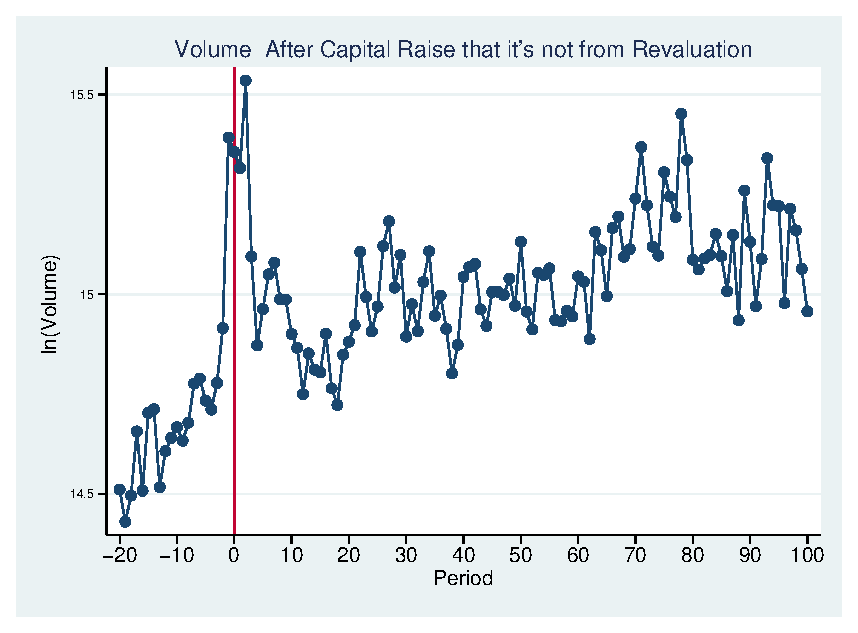
\includegraphics[width=0.7\linewidth]{volume_NoRevaluation}
\label{fig:volumenorevaluation}
\end{figure}
\end{frame}


\subsection{Relative Volume}
\begin{frame}{Relative volume}
\begin{figure}
\centering
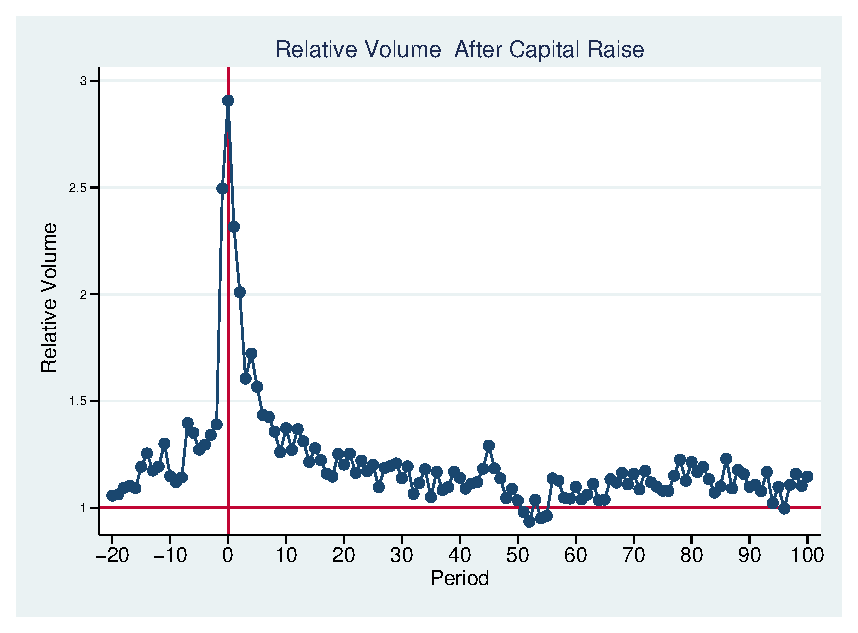
\includegraphics[width=0.7\linewidth]{Relvolume}
\label{fig:relvolume}
\end{figure}
\end{frame}
\begin{frame}{Relative volume}{Relative Volume of raised capital from Revaluation}
\begin{figure}
\centering
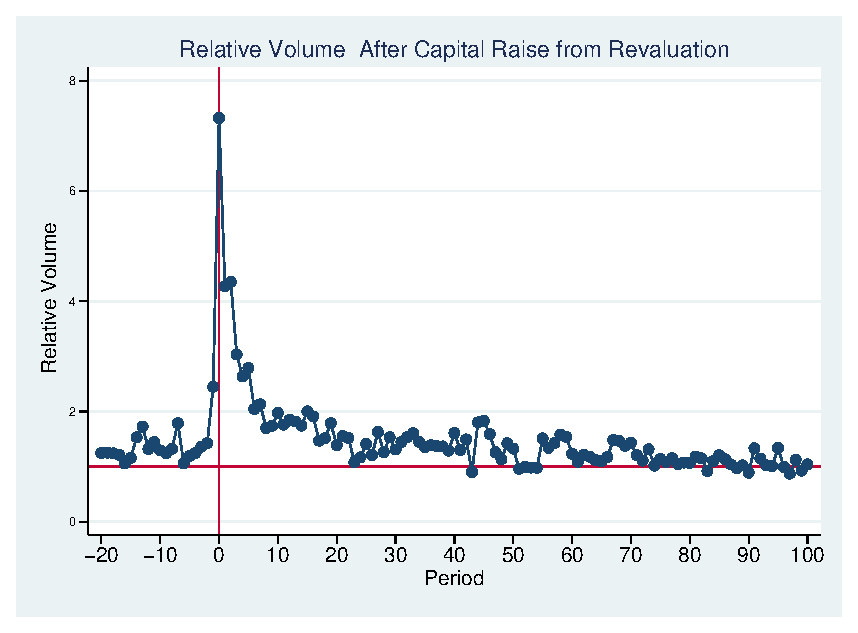
\includegraphics[width=0.7\linewidth]{Relvolume_Revaluation}
\label{fig:relvolumerevaluation}
\end{figure}
\end{frame}
\begin{frame}{Relative volume}{Relative Volume of raised capital that it's not from Revaluation}
\begin{figure}
\centering
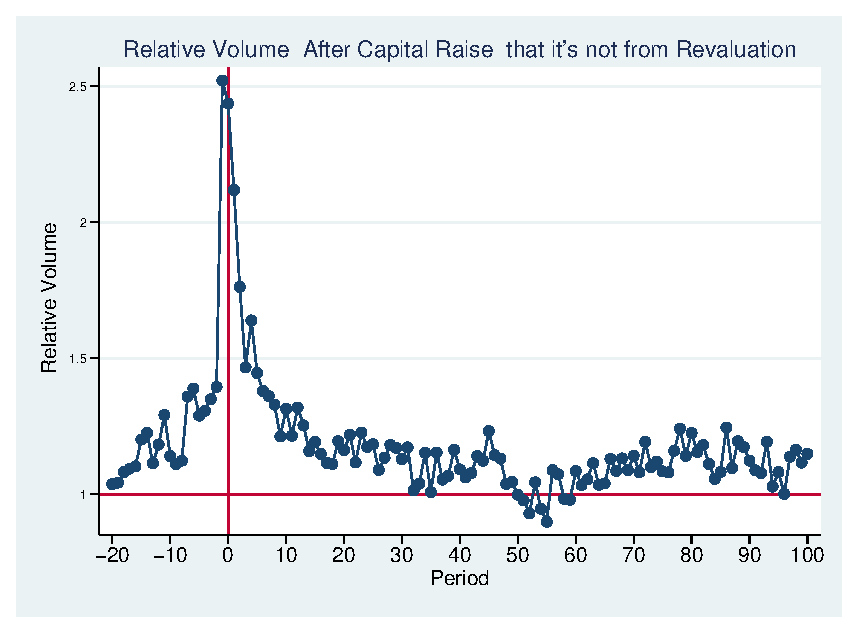
\includegraphics[width=0.7\linewidth]{Relvolume_NoRevaluation}
\label{fig:relvolumenorevaluation}
\end{figure}
\end{frame}



\subsection{Buy-sell Imbalances}

\begin{frame}{Buy-sell Imbalances}
\begin{figure}
\centering
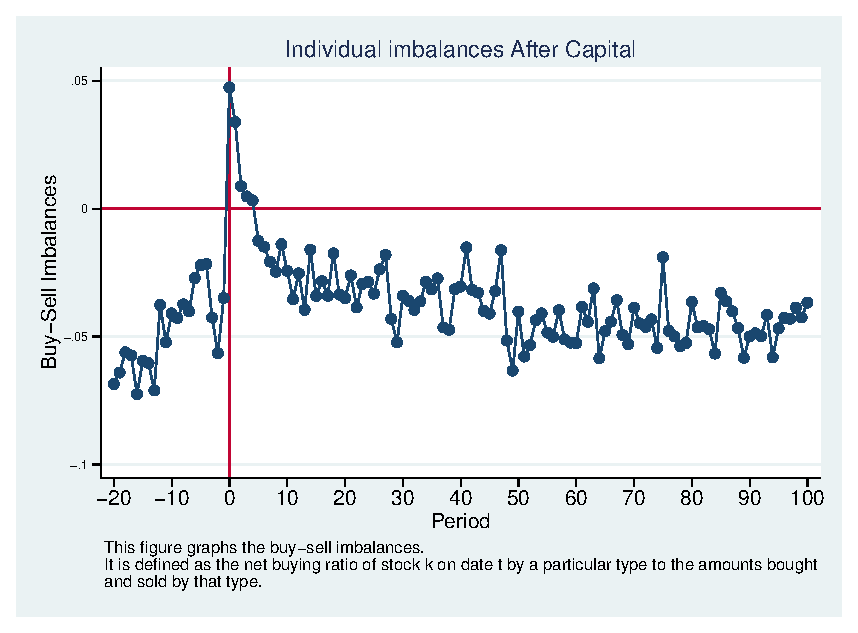
\includegraphics[width=0.45\linewidth]{IndImb}
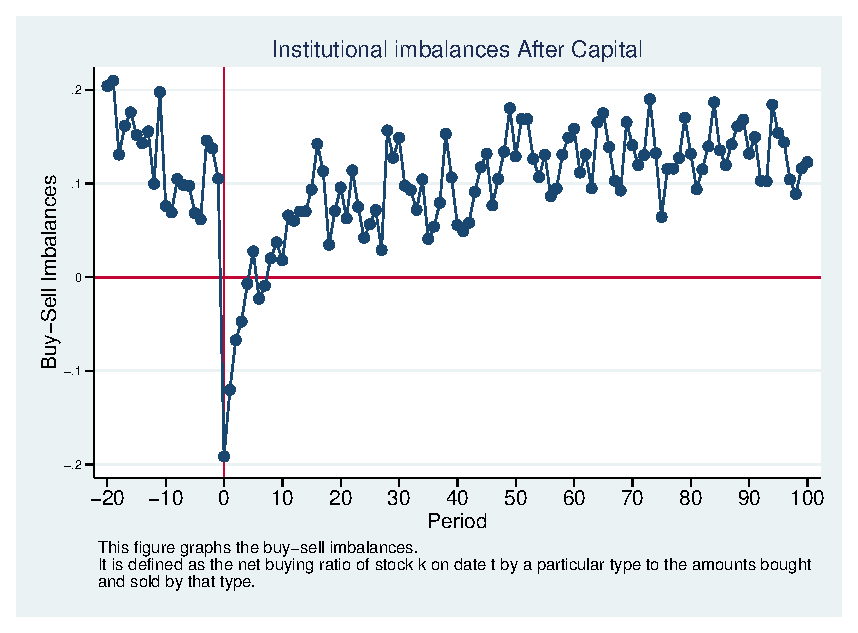
\includegraphics[width=0.45\linewidth]{InsImb}
\label{fig:indimb}
\end{figure}
\end{frame}
\begin{frame}{Buy-sell Imbalances}{Buy-sell Imbalances of raised capital from Revaluation}
\begin{figure}
\centering
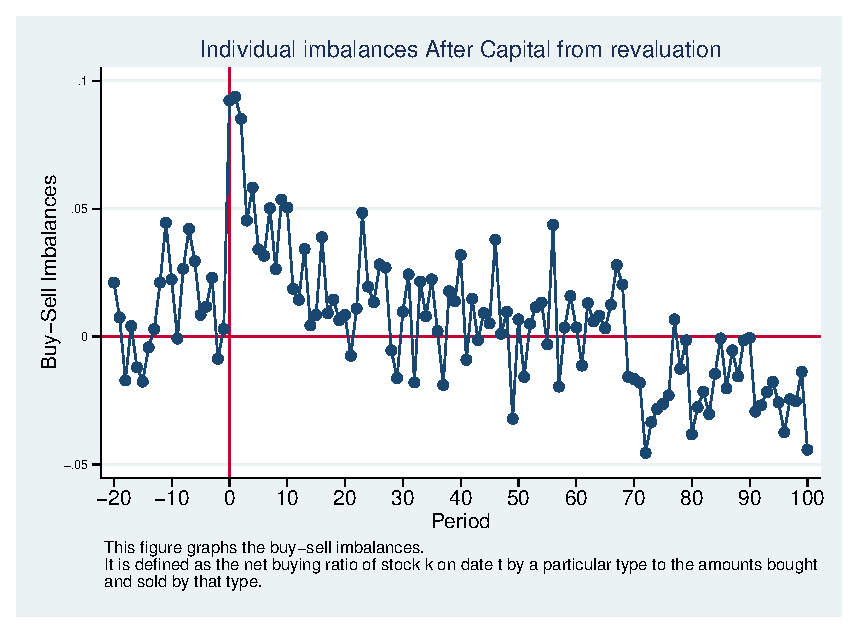
\includegraphics[width=0.45\linewidth]{IndImb_Revaluation}
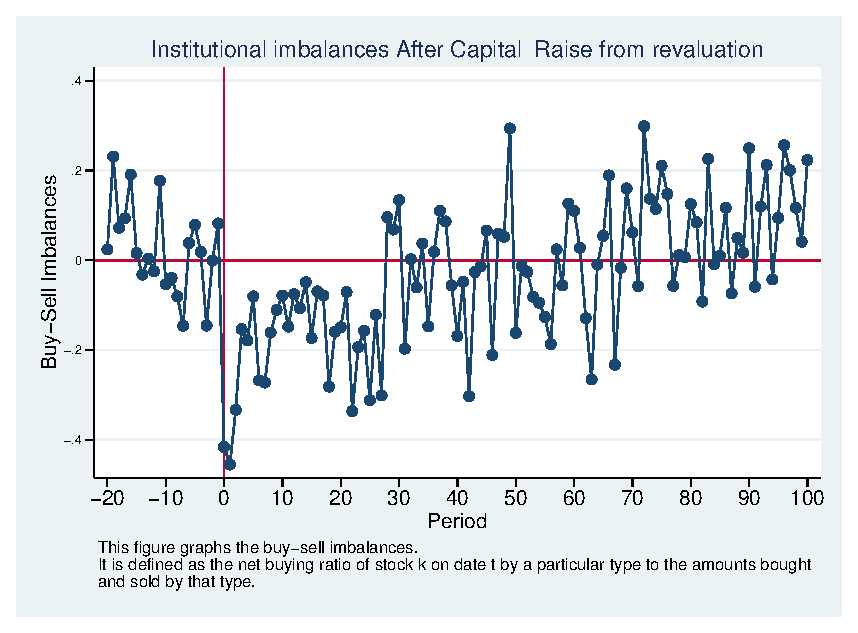
\includegraphics[width=0.45\linewidth]{InsImb_Revaluation}
\label{fig:indimbrevaluation}
\end{figure}
\end{frame}
\begin{frame}{Buy-sell Imbalances}{Buy-sell Imbalances of raised capital that it's not from Revaluation}
\begin{figure}
\centering
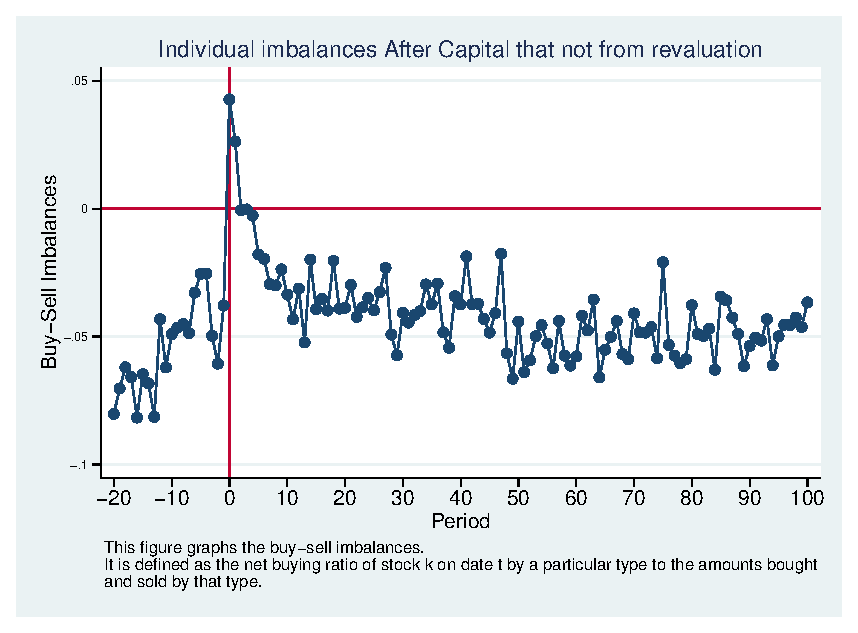
\includegraphics[width=0.45\linewidth]{IndImb_NoRevaluation}
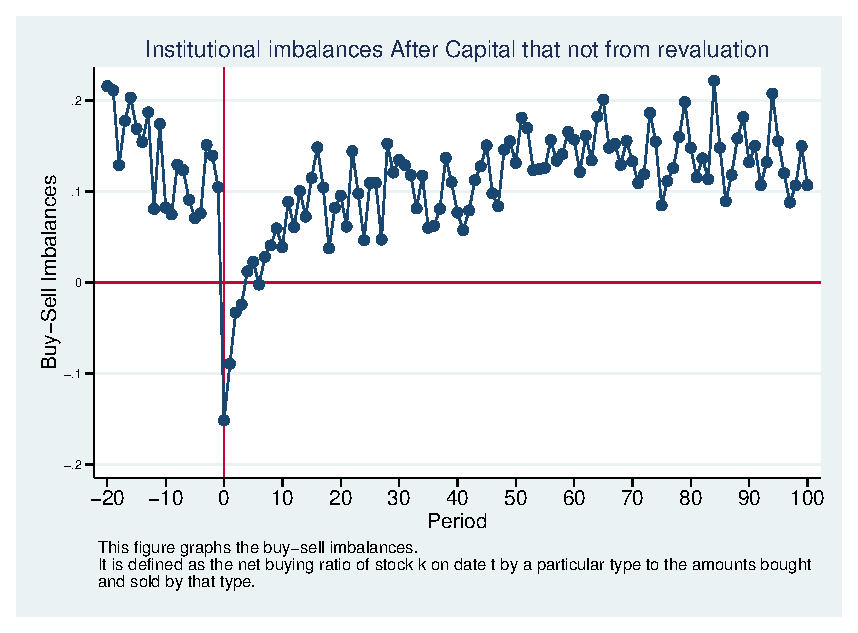
\includegraphics[width=0.45\linewidth]{InsImb_NoRevaluation}
\label{fig:indimbnorevaluation}
\end{figure}
\end{frame}


























\section{Abnormal Return Analysis}
\def\sym#1{\ifmmode^{#1}\else\(^{#1}\)\fi}
\begin{frame}
\begin{center}

\begin{columns}

\column{.5\textwidth}     
 \centering
 \resizebox{0.7\textwidth}{!}{
         \begin{tabular}{CCCC}
         \toprule\toprule
         \multicolumn{4}{c}{\textit{Abnormal Return at event day }} \\
                \multicolumn{4}{c}{\scriptsize\textit{Panel A:}{ Market Cap}}\\
                \hline\hline
               & \multicolumn{2}{c}{\scriptsize Revaluation}        &  \\
               \cmidrule{2-3}
         \multicolumn{1}{l}{Sub sample} & \multicolumn{1}{c}{No} & \multicolumn{1}{c}{Yes} & \multicolumn{1}{c}{Total} \\
          \hline
    \rowfont{\normalsize}%
    Small & 6.73  & 39.64 & 9.48 \\
    \rowfont{\scriptsize}%
      sd    & 19.66 & 40.16 & 23.82 \\
        n  & 285   & 26    & 311 \\
          \hline
    \rowfont{\normalsize}%      
    Middle & 3.73  & 37.33 & 6.47 \\
    \rowfont{\scriptsize}%
       sd   & 12.88 & 41.20 & 19.24 \\
       n  & 282   & 25    & 307 \\
          \hline
          \rowfont{\normalsize}%
    Large & 2.37  & 12.68 & 3.38 \\
    \rowfont{\scriptsize}%
       sd   & 11.21 & 16.96 & 12.26 \\
       n   & 293   & 32    & 325 \\
          \hline
          \rowfont{\normalsize}%
    Full sample & 4.26  & 28.55 & 6.40 \\
    \rowfont{\scriptsize}%
      sd    & 15.11 & 35.47 & 19.10 \\
       n   & 860   & 83    & 943 \\
          \hline
          \rowfont{\normalsize}%
    Small - Large & 4.366\sym{***} & 26.96\sym{**} & 6.101\sym{***} \\
   \scriptsize P-Value & 0.001 & 0.003 & 0 \\
     \bottomrule\bottomrule
     \addlinespace[.75ex]
     \end{tabular}
 }
 
 \column{.5\textwidth}     
  \centering
   \resizebox{0.58\textwidth}{!}{
      \begin{tabular}{CCCC}
               \toprule\toprule
               \multicolumn{4}{c}{\textit{Abnormal Return at event day }} \\
                      \multicolumn{4}{c}{\scriptsize\textit{Panel B:} {P/E ratio}}\\
                      \hline\hline
                     & \multicolumn{2}{c}{\scriptsize Revaluation}        &  \\
                     \cmidrule{2-3}
               \multicolumn{1}{l}{Sub sample} & \multicolumn{1}{c}{No} & \multicolumn{1}{c}{Yes} & \multicolumn{1}{c}{Total} \\
                \hline
                \rowfont{\normalsize}%
   {Low} & 2.39  & 35.88 & 4.99 \\
   \rowfont{\scriptsize}%
       sd   & 15.22 & 42.50 & 20.67 \\
        n  & 214   & 18    & 232 \\\hline\rowfont{\normalsize}%
    {Middle} & 4.76  & 37.58 & 7.07 \\
       sd   & 20.26 & 41.74 & 23.84 \\
        n  & 224   & 17    & 241 \\\hline\rowfont{\normalsize}%
    {High} & 3.83  & 18.20 & 5.14 \\\rowfont{\scriptsize}%
       sd   & 9.95  & 23.17 & 12.41 \\
       n   & 219   & 22    & 241 \\\hline\rowfont{\normalsize}%
    {Full sample} & 3.68  & 29.56 & 5.74 \\\rowfont{\scriptsize}%
       sd   & 15.77 & 36.48 & 19.56 \\
       n   & 657   & 57    & 714 \\ 
          \hline \rowfont{\normalsize}%
    {Low - High} & -1.436 & 17.68 & -0.149 \\\rowfont{\scriptsize}%
    {P-Value}     & 0.247 & 0.126 & 0.924 \\           
           \bottomrule\bottomrule
           \addlinespace[.75ex]
           \end{tabular}
       }


 
\end{columns}

\normalsize
\end{center}
\end{frame}


\begin{frame}
\begin{center}

\begin{columns}
\column{.5\textwidth}     
 \centering
 
  \resizebox{0.6\textwidth}{!}{
          \begin{tabular}{CCCC}
          \toprule\toprule
          \multicolumn{4}{c}{\textit{Abnormal Return at event day }} \\
                 \multicolumn{4}{c}{\scriptsize\textit{Panel C:}{ Book-to-Market}}\\
                 \hline\hline
                & \multicolumn{2}{c}{\scriptsize Revaluation}        &  \\
                \cmidrule{2-3}
          \multicolumn{1}{l}{Sub sample} & \multicolumn{1}{c}{No} & \multicolumn{1}{c}{Yes} & \multicolumn{1}{c}{Total} \\
           \hline\rowfont{\normalsize}%
          {Low} & 5.48  & 36.85 & 8.08 \\\rowfont{\scriptsize}%
            sd    & 19.07 & 47.28 & 24.23 \\
             n   & 288   & 26    & 314 \\
                 \hline\rowfont{\normalsize}%
          {Middle} & 3.14  & 28.41 & 5.03 \\\rowfont{\scriptsize}%
             sd   & 12.87 & 33.15 & 16.62 \\
             n   & 285   & 23    & 308 \\
                 \hline\rowfont{\normalsize}%
          {High} & 4.15  & 22.30 & 6.07 \\\rowfont{\scriptsize}%
             sd   & 12.38 & 24.60 & 15.18 \\
             n   & 287   & 34    & 321 \\
                 \hline\rowfont{\normalsize}%
          {Full sample} & 4.26  & 28.55 & 6.40 \\\rowfont{\scriptsize}%
             sd   & 15.11 & 35.47 & 19.10 \\
              n  & 860   & 83    & 943 \\
                \hline\rowfont{\normalsize}%
         {Low - High} & 1.327 & 14.55 & 2.003 \\\rowfont{\scriptsize}%
          {P-Value}      & 0.323 & 0.162 & 0.214 \\
      \bottomrule\bottomrule
      \addlinespace[.75ex]
      \end{tabular}
  }
  
  
 
 \column{.5\textwidth}     
  \centering
   \resizebox{0.6\textwidth}{!}{
      \begin{tabular}{CCCC}
               \toprule\toprule
               \multicolumn{4}{c}{\textit{Abnormal Return at event day }} \\
                      \multicolumn{4}{c}{\scriptsize\textit{Panel D:}{ Free Float}}\\
                      \hline\hline
                     & \multicolumn{2}{c}{\scriptsize Revaluation}        &  \\
                     \cmidrule{2-3}
               \multicolumn{1}{l}{Sub sample} & \multicolumn{1}{c}{No} & \multicolumn{1}{c}{Yes} & \multicolumn{1}{c}{Total} \\
                \hline\rowfont{\normalsize}%
    Low   & 5.13  & 21.17 & 6.59 \\\rowfont{\scriptsize}%
      sd    & 19.60 & 23.58 & 20.48 \\
        n  & 271   & 27    & 298 \\\hline\rowfont{\normalsize}%
    Middle & 3.39  & 28.43 & 5.31 \\\rowfont{\scriptsize}%
       sd   & 12.62 & 41.21 & 17.79 \\
       n   & 277   & 23    & 300 \\\hline\rowfont{\normalsize}%
    High  & 4.20  & 35.52 & 7.32 \\\rowfont{\scriptsize}%
       sd   & 12.45 & 39.95 & 19.54 \\
        n  & 281   & 31    & 312 \\\hline\rowfont{\normalsize}%
    Full sample & 4.24  & 28.72 & 6.42 \\
        sd  & 15.21 & 35.83 & 19.30 \\\rowfont{\scriptsize}%
        n  & 829   & 81    & 910 \\
          \hline\rowfont{\normalsize}%
    Low - High &  0.929 & -14.35 & -0.73 \\\rowfont{\scriptsize}%
    P-Value &0.508  &  0.097 & 0.653 \\        
           \bottomrule\bottomrule
           \addlinespace[.75ex]
           \end{tabular}
       }
\end{columns}

\normalsize
\end{center}
\end{frame}




\begin{frame}
\begin{center}

\begin{columns}
\column{.5\textwidth}     
 \centering
 \resizebox{0.75\textwidth}{!}{
         \begin{tabular}{CCCC}
         \toprule\toprule
         \multicolumn{4}{c}{\textit{Abnormal Return at event day }} \\
                \multicolumn{4}{c}{\scriptsize\textit{Panel E: }{ Free Market Cap}}\\
                \hline\hline
               & \multicolumn{2}{c}{\scriptsize Revaluation}        &  \\
               \cmidrule{2-3}
         \multicolumn{1}{l}{Sub sample} & \multicolumn{1}{c}{No} & \multicolumn{1}{c}{Yes} & \multicolumn{1}{c}{Total} \\
          \hline\rowfont{\normalsize}
    Small & 6.11  & 40.98 & 9.36 \\\rowfont{\scriptsize}
       sd   & 20.10 & 46.67 & 25.81 \\
       n   & 272   & 28    & 300 \\ \hline\rowfont{\normalsize}
    Middle & 4.39  & 27.42 & 6.11 \\\rowfont{\scriptsize}
       sd   & 13.36 & 30.56 & 16.39 \\
        n  & 273   & 22    & 295 \\ \hline\rowfont{\normalsize}
    Large & 2.30  & 18.58 & 3.90 \\\rowfont{\scriptsize}
       sd   & 10.54 & 23.67 & 13.31 \\
       n   & 284   & 31    & 315 \\ \hline\rowfont{\normalsize}
    Full sample & 4.24  & 28.72 & 6.42 \\\rowfont{\scriptsize}
       sd   & 15.21 & 35.83 & 19.30 \\
       n   & 829   & 81    & 910 \\ \hline\rowfont{\normalsize}
    Small - Large & 3.813\sym{**} & 22.41\sym{***} & 5.466\sym{***} \\\rowfont{\scriptsize}
    P-Value & 0.006 & 0.028 & 0.001 \\
     \bottomrule\bottomrule
     \addlinespace[.75ex]
     \end{tabular}
 }
 
 
 \column{.5\textwidth}     
  \centering
   \resizebox{0.6\textwidth}{!}{
      \begin{tabular}{CCCC}
               \toprule\toprule
               \multicolumn{4}{c}{\textit{Abnormal Return at event day }} \\
                      \multicolumn{4}{c}{\scriptsize\textit{Panel F:}{ Volatility(past 250 days)}}\\
                      \hline\hline
                     & \multicolumn{2}{c}{\scriptsize Revaluation}        &  \\
                     \cmidrule{2-3}
               \multicolumn{1}{l}{Sub sample} & \multicolumn{1}{c}{No} & \multicolumn{1}{c}{Yes} & \multicolumn{1}{c}{Total} \\
                \hline\rowfont{\normalsize}
    Low   & 4.50  & 24.11 & 6.29 \\\rowfont{\scriptsize}
      sd    & 18.72 & 28.69 & 20.56 \\
       n   & 269   & 27    & 296 \\\hline\rowfont{\normalsize}
    Middle & 4.90  & 34.68 & 7.32 \\\rowfont{\scriptsize}
        sd  & 12.28 & 33.07 & 17.04 \\
       n   & 260   & 23    & 283 \\\hline\rowfont{\normalsize}
    High  & 2.68  & 23.08 & 4.82 \\\rowfont{\scriptsize}
       sd   & 13.92 & 34.70 & 18.31 \\
       n   & 264   & 31    & 295 \\\hline\rowfont{\normalsize}
    Full sample & 4.02  & 26.72 & 6.13 \\\rowfont{\scriptsize}
      sd    & 15.27 & 32.33 & 18.73 \\
       n   & 793   & 81    & 874 \\\hline\rowfont{\normalsize}
    Low - High & 1.823 & 1.037 & 1.468 \\\rowfont{\scriptsize}
    P-Value & 0.202 & 0.901 & 0.36 \\      
           \bottomrule\bottomrule
           \addlinespace[.75ex]
           \end{tabular}
       }
\end{columns}


\normalsize
\end{center}
\end{frame}



\begin{frame}
\begin{center}

\begin{columns}
\column{.5\textwidth}     
 \centering
 \resizebox{0.6\textwidth}{!}{
         \begin{tabular}{CCCC}
         \toprule\toprule
         \multicolumn{4}{c}{\textit{Abnormal Return at event day }} \\
                \multicolumn{4}{c}{\scriptsize\textit{Panel G: }{Debt ratio}}\\
                \hline\hline
               & \multicolumn{2}{c}{\scriptsize Revaluation}        &  \\
               \cmidrule{2-3}
         \multicolumn{1}{l}{Sub sample} & \multicolumn{1}{c}{No} & \multicolumn{1}{c}{Yes} & \multicolumn{1}{c}{Total} \\
          \hline\rowfont{\normalsize}
    Low   & 4.19  & 34.87 & 6.80 \\\rowfont{\scriptsize}
      sd    & 18.95 & 43.56 & 23.61 \\
       n   & 280   & 26    & 306 \\\hline\rowfont{\normalsize}
    Middle & 3.69  & 28.19 & 5.67 \\\rowfont{\scriptsize}
       sd   & 11.93 & 25.80 & 15.07 \\
       n   & 273   & 24    & 297 \\\hline\rowfont{\normalsize}
    High  & 5.06  & 23.42 & 6.80 \\\rowfont{\scriptsize}
       sd   & 14.24 & 36.81 & 18.36 \\
        n  & 277   & 29    & 306 \\\hline\rowfont{\normalsize}
    Full sample & 4.32  & 28.64 & 6.43 \\\rowfont{\scriptsize}
       sd   & 15.34 & 36.25 & 19.36 \\
       n   & 830   & 79    & 909 \\\hline\rowfont{\normalsize}
    Low - High & -0.872 & 11.45 & -0.005 \\\rowfont{\scriptsize}
    P-Value & 0.539 & 0.301 & 0.998 \\
     \bottomrule\bottomrule
     \addlinespace[.75ex]
     \end{tabular}
 }
 
 
 \column{.5\textwidth}     
  \centering
   \resizebox{0.6\textwidth}{!}{
      \begin{tabular}{CCCC}
               \toprule\toprule
               \multicolumn{4}{c}{\textit{Abnormal Return at event day }} \\
                      \multicolumn{4}{c}{\scriptsize\textit{Panel H:}{ Leverage ratio}}\\
                      \hline\hline
                     & \multicolumn{2}{c}{\scriptsize Revaluation}        &  \\
                     \cmidrule{2-3}
               \multicolumn{1}{l}{Sub sample} & \multicolumn{1}{c}{No} & \multicolumn{1}{c}{Yes} & \multicolumn{1}{c}{Total} \\
                \hline\rowfont{\normalsize}
    Low   & 3.80  & 29.24 & 5.97 \\\rowfont{\scriptsize}
      sd    & 10.37 & 31.09 & 15.13 \\
       n   & 278   & 26    & 304 \\\hline\rowfont{\normalsize}
    Middle & 3.84  & 23.49 & 5.36 \\\rowfont{\scriptsize}
       sd   & 12.64 & 29.34 & 15.46 \\
       n   & 274   & 23    & 297 \\\hline\rowfont{\normalsize}
    High  & 5.31  & 32.06 & 7.92 \\\rowfont{\scriptsize}
      sd    & 20.93 & 44.88 & 25.47 \\
      b    & 278   & 30    & 308 \\\hline\rowfont{\normalsize}
    Full sample & 4.32  & 28.64 & 6.43 \\\rowfont{\scriptsize}
       sd   & 15.34 & 36.25 & 19.36 \\
       n   & 830   & 79    & 909 \\\hline\rowfont{\normalsize}
    Low - High & -1.512 & -2.817 & -1.941 \\\rowfont{\scriptsize}
    P-Value & 0.281 & 0.784 & 0.251 \\      
           \bottomrule\bottomrule
           \addlinespace[.75ex]
           \end{tabular}
       }
\end{columns}


\normalsize
\end{center}
\end{frame}


\begin{frame}
\begin{center}

 \resizebox{0.25\textwidth}{!}{
         \begin{tabular}{CCCC}
         \toprule\toprule
         \multicolumn{4}{c}{\textit{Abnormal Return at event day }} \\
                \multicolumn{4}{c}{\scriptsize\textit{Panel I: }{Market Condition}}\\
                \hline\hline
               & \multicolumn{2}{c}{\scriptsize Revaluation}        &  \\
               \cmidrule{2-3}
         \multicolumn{1}{l}{Sub sample} & \multicolumn{1}{c}{No} & \multicolumn{1}{c}{Yes} & \multicolumn{1}{c}{Total} \\
          \hline\rowfont{\normalsize}
    {Bad} & 3.85  & 29.85 & 6.20 \\\rowfont{\scriptsize}
      sd    & 12.96 & 37.65 & 18.25 \\
        n  & 301   & 30    & 331 \\\hline\rowfont{\normalsize}
    {Good} & 4.48  & 27.82 & 6.51 \\\rowfont{\scriptsize}
       sd   & 16.15 & 34.52 & 19.56 \\
        n  & 559   & 53    & 612 \\\hline\rowfont{\normalsize}
    {Full sample} & 4.26  & 28.55 & 6.40 \\\rowfont{\scriptsize}
        sd  & 15.11 & 35.47 & 19.10 \\
        n  & 860   & 83    & 943 \\
     \bottomrule\bottomrule
     \addlinespace[.75ex]
     \end{tabular}
 }


\normalsize
\end{center}
\end{frame}


%\begin{frame}
%\begin{center}
%\footnotesize
%\newcolumntype{Y}{>{\raggedleft\arraybackslash}X}
%\resizebox{0.8\textwidth}{!}{
%\begin{tabularx} {15cm} {@{}  l Y Y Y Y Y Y@{}} 
%\toprule\toprule
%\multicolumn{7}{c}{\textit{Mean of Abnormal Return}} \\
%\hline\hline
% & \multicolumn{6}{c}{\scriptsize P/E Quantile} \\
%\cmidrule{2-6} \scriptsize Size Quantile&$ 1_\text{\tiny (Low)} $&2&3&4&$ 5_\text{\tiny (High)} $&Row average \\
%\hline
%$ 1_\text{\tiny (Low)} $&17.0&11.8&29.9&8.5&7.9&13.3 \\
%2&15.0&8.1&3.0&8.7&5.4&8.0 \\
%3&0.3&-0.5&5.3&6.5&6.8&4.0 \\
%4&-2.3&2.2&-1.1&3.0&3.1&0.9 \\
%$ 5_\text{\tiny (High)} $&2.4&-0.4&3.6&1.1&7.5&2.6 \\
%Column average&7.1&3.3&5.1&5.7&6.0&5.4 \\
%
%\bottomrule\bottomrule
%\addlinespace[.75ex]
%\end{tabularx}
%}
%\par
%
%\normalsize
%\end{center}
%\end{frame}
%
%\begin{frame}
%
%\begin{center}
%\footnotesize
%\newcolumntype{Y}{>{\raggedleft\arraybackslash}X}
%\resizebox{0.8 \textwidth}{!}{
%\begin{tabularx} {15cm} {@{} l Y Y Y Y Y Y@{}} 
%\toprule \toprule
%\multicolumn{7}{c}{\textit{Mean of Abnormal Return}} \\
%\hline\hline
% & \multicolumn{6}{c}{\scriptsize Book-to-Market Quantile} \\
%\cmidrule{2-6} \scriptsize P/E Quantile &$ 1_\text{\tiny (Low)} $&2&3&4&$ 5_\text{\tiny (High)} $&Row average \\
%\hline
%$ 1_\text{\tiny (Low)} $&15.4&3.3&3.7&6.3&4.6&7.1 \\
%2&4.0&2.9&5.1&2.0&1.6&3.3 \\
%3&11.8&4.3&1.5&2.5&4.2&5.1 \\
%4&4.8&6.5&2.8&8.6&5.5&5.7 \\
%$ 5_\text{\tiny (High)} $&10.2&7.0&2.9&4.8&5.9&6.0 \\
%Column average&9.6&4.7&3.3&4.6&4.8&5.4 \\
%\bottomrule
%\bottomrule
%\addlinespace[.75ex]
%\end{tabularx}
%}
%\par
%\normalsize
%\end{center}
%
%\end{frame}





%\begin{frame}
%\begin{table}[htbp]
%\centering
%    \resizebox{0.4\textheight}{!}{
%{
\def\sym#1{\ifmmode^{#1}\else\(^{#1}\)\fi}
\begin{tabular}{l*{4}{c}}
\hline\hline
                &\multicolumn{2}{c}{CAPM}             &\multicolumn{2}{c}{4Factor}          \\\cmidrule(lr){2-3}\cmidrule(lr){4-5}
                &\multicolumn{1}{c}{(1)}         &\multicolumn{1}{c}{(2)}         &\multicolumn{1}{c}{(3)}         &\multicolumn{1}{c}{(4)}         \\
\hline
Bullish Market  &    1.803         &    1.668         &    1.992         &    1.694         \\
                &   (1.11)         &   (1.22)         &   (1.18)         &   (1.15)         \\
[1em]
High Book-to-Market&    2.395         &    1.877         &    1.922         &    1.529         \\
                &   (1.53)         &   (1.44)         &   (1.23)         &   (1.19)         \\
[1em]
High P/E        &    0.225         &                  &   -0.416         &                  \\
                &   (0.13)         &                  &  (-0.22)         &                  \\
[1em]
Large           &   -7.073\sym{*}  &   -4.872\sym{*}  &   -7.013\sym{*}  &   -4.424         \\
                &  (-2.64)         &  (-2.25)         &  (-2.27)         &  (-1.82)         \\
[1em]
High Free Float &    0.197         &   -0.226         &    0.102         &   -0.761         \\
                &   (0.17)         &  (-0.20)         &   (0.08)         &  (-0.58)         \\
[1em]
High Free Market Cap&    0.965         &   -0.152         &    1.056         &    0.137         \\
                &   (0.34)         &  (-0.06)         &   (0.33)         &   (0.05)         \\
[1em]
High Volatility &   -3.391         &   -2.141         &   -3.732         &   -2.115         \\
                &  (-1.68)         &  (-1.35)         &  (-1.74)         &  (-1.25)         \\
[1em]
High Debt Ratio &   -2.391         &   -0.334         &   -1.738         &   -0.377         \\
                &  (-0.81)         &  (-0.16)         &  (-0.58)         &  (-0.18)         \\
[1em]
High Leverage Ratio&    2.964         &    1.401         &    2.470         &    0.872         \\
                &   (0.94)         &   (0.60)         &   (0.78)         &   (0.36)         \\
[1em]
Resereves       &    2.182         &    2.153         &    1.477         &    1.607         \\
                &   (1.01)         &   (1.19)         &   (0.70)         &   (0.88)         \\
[1em]
Cash \& Resereves&    2.814         &    2.478         &    2.316         &    2.490         \\
                &   (1.71)         &   (1.73)         &   (1.44)         &   (1.67)         \\
[1em]
Revaluation     &    26.02\sym{***}&    21.69\sym{***}&    27.77\sym{***}&    24.74\sym{***}\\
                &   (4.44)         &   (4.38)         &   (4.40)         &   (4.89)         \\
[1em]
Constant        &    4.589         &    4.317\sym{*}  &    5.063         &    4.068         \\
                &   (1.61)         &   (2.21)         &   (1.61)         &   (1.90)         \\
\hline
Observations    &      651         &      857         &      651         &      857         \\
\hline\hline
\multicolumn{5}{l}{\footnotesize \textit{t} statistics in parentheses}\\
\multicolumn{5}{l}{\footnotesize \sym{*} \(p<0.05\), \sym{**} \(p<0.01\), \sym{***} \(p<0.001\)}\\
\end{tabular}
}

%}
%\end{table}
%\end{frame}


	\tiny
\begin{frame}[allowframebreaks]{References}
	
	{		
		\bibliographystyle{apalike}
		\bibliography{Ref}
	}
\end{frame}

\normalsize


\appendix






\section{Appendix I : 4 Factor Abnormal Return}
\begin{frame}{Abnormal Return}
\label{abreturn4Factor}
\begin{figure}
\centering
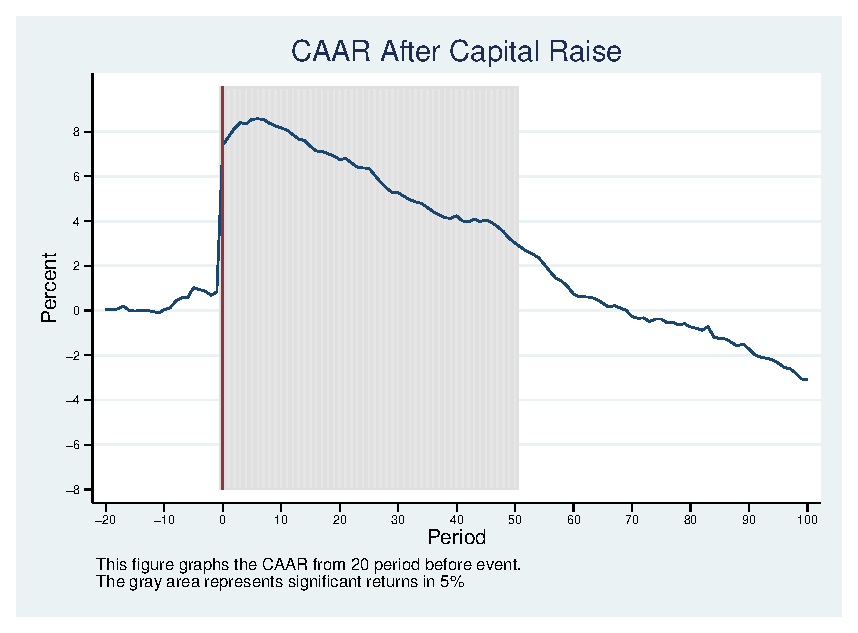
\includegraphics[width=0.7\linewidth]{AbReturn_4Factor.eps}
\label{fig:abreturn2}
\end{figure}
\hfill\hyperlink{abreturn}{\beamerbutton{CAPM}}
\end{frame}

\begin{frame}{Abnormal Return}{Abnormal return of raised capital from Revaluation}
\label{abreturnrevalution4Factor}
\begin{figure}
\centering
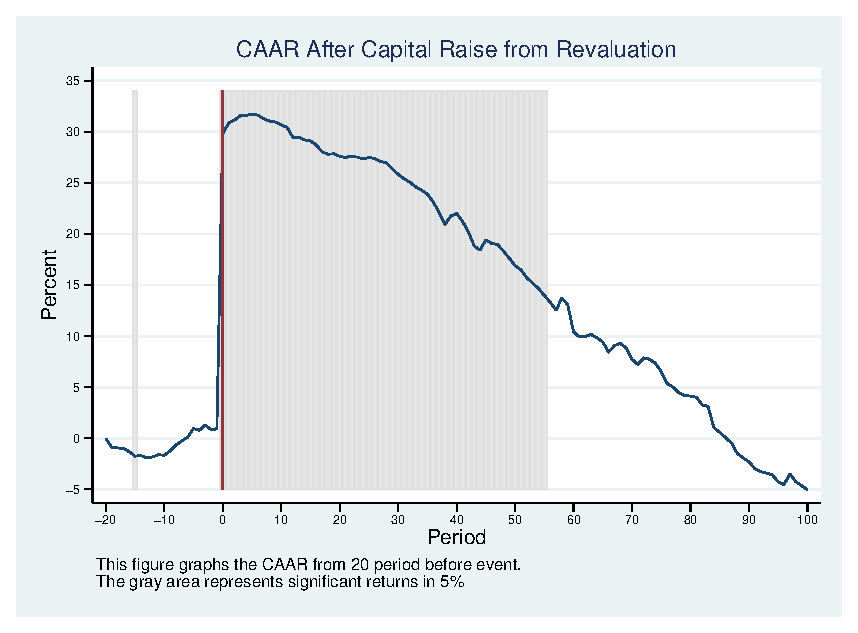
\includegraphics[width=0.65\linewidth]{AbReturnRevalution_4Factor}
\label{fig:abreturnrevalution2}
\end{figure}

\hfill\hyperlink{abreturnrevalution}{\beamerbutton{CAPM}}
\end{frame}


\begin{frame}{Abnormal Return}{Abnormal return of raised capital from Reserves}
\label{abreturnsaving4Factor}
\begin{figure}
\centering
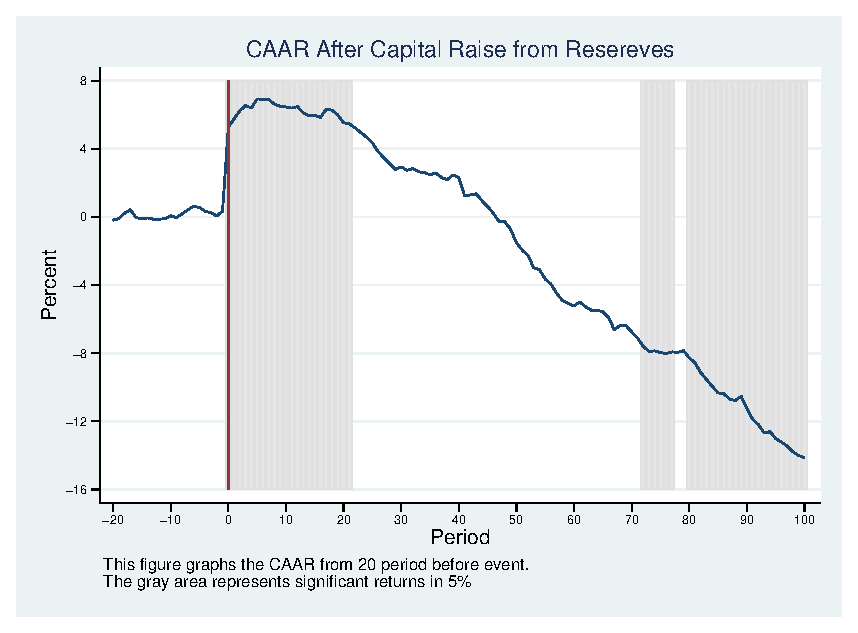
\includegraphics[width=0.65\linewidth]{AbReturnSaving_4Factor}
\label{fig:abreturnsaving2}
\end{figure}

\hfill\hyperlink{abreturnsaving}{\beamerbutton{CAPM}}
\end{frame}


\begin{frame}{Abnormal Return}{Abnormal return of raised capital from Cash}
\label{abreturncash4Factor}
\begin{figure}
\centering
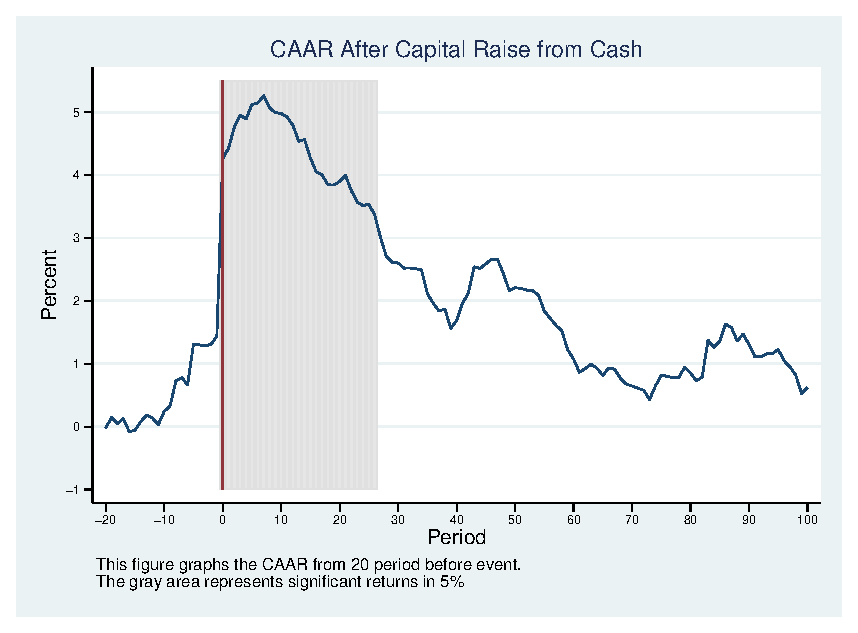
\includegraphics[width=0.65\linewidth]{AbReturnCash_4Factor}
\label{fig:abreturncash2}
\end{figure}
\hfill\hyperlink{abreturncash}{\beamerbutton{CAPM}}
\end{frame}


\begin{frame}{Abnormal Return}{Abnormal return of raised capital from Cash \& Reserves}
\label{abreturnhybrid4Factor}
\begin{figure}
\centering
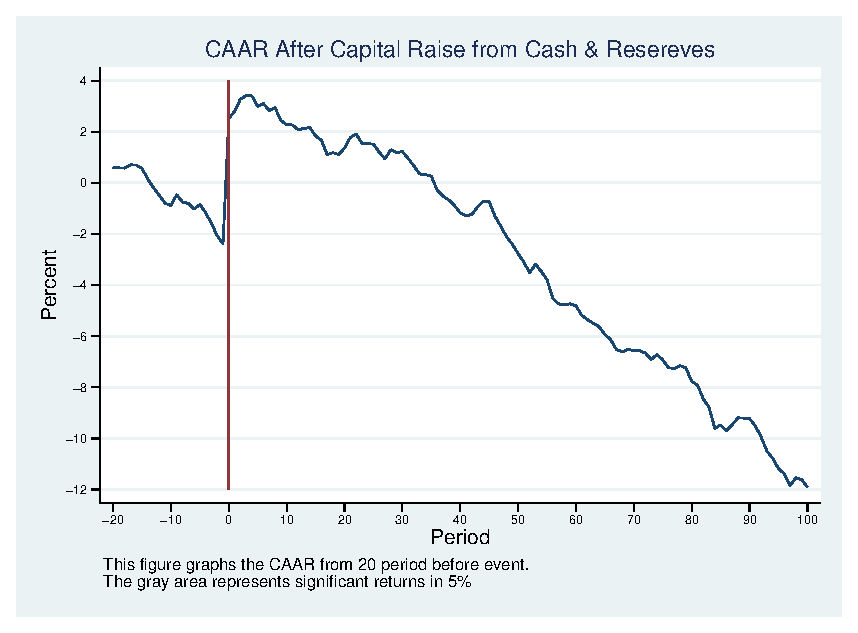
\includegraphics[width=0.65\linewidth]{AbReturnHybrid_4Factor}
\label{fig:abreturnhybrid2}
\end{figure}
\hfill\hyperlink{abreturnhybrid}{\beamerbutton{CAPM}}
\end{frame}


\section{Appendix II : CAPM ($ \alpha = 0 $)}

\begin{frame}
\begin{block}{\footnotesize Brooks, Chris. Introductory econometrics for finance. Cambridge university press, 2019}
\scriptsize
An interesting question is whether the expected return should
incorporate the $ \alpha $ from the estimation period in addition to $ \beta $ multiplied by the market return.
 Most applications of event studies include this, and indeed the original study by Fama et al. (1969) includes an alpha.
 
However, we need to exercise caution when doing so since if – either
because of some unrelated incident affecting the price of the stock or in
anticipation of the event – the alpha is particularly high (particularly low) during the estimation period, it will push up (down) the expected return.
Thus it may be preferable to assume an expected value of zero for the
alpha and to exclude it from the event period abnormal return calculation.
\end{block}
\end{frame}

\begin{frame}{Abnormal Return}
\label{abreturnWithoutAlpha}
\begin{figure}
\centering
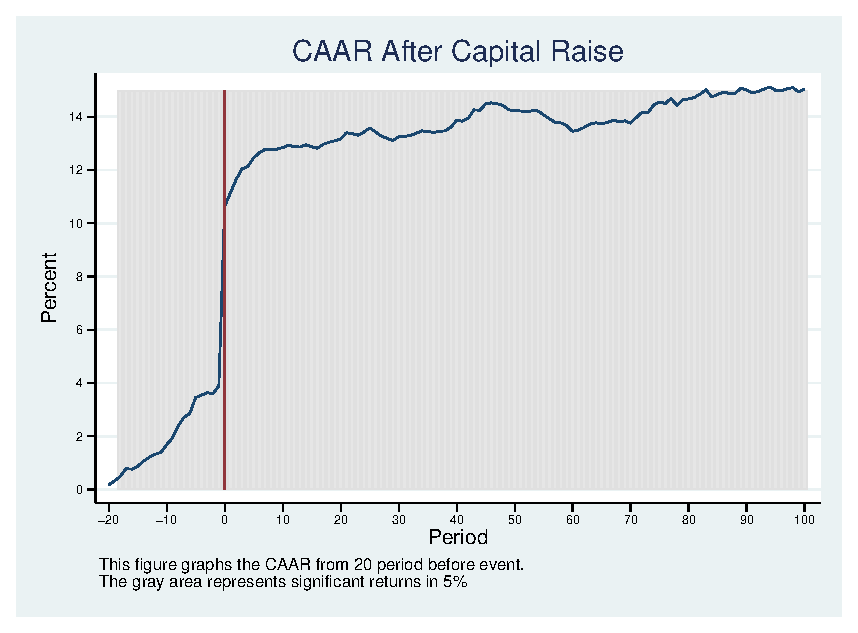
\includegraphics[width=0.7\linewidth]{AbReturn_WithoutAlpha.eps}
\label{fig:abreturn3}
\end{figure}
\hfill\hyperlink{abreturn}{\beamerbutton{CAPM}}
\end{frame}

\begin{frame}{Abnormal Return}{Abnormal return of raised capital from Revaluation}
\label{abreturnrevalutionWithoutAlpha}
\begin{figure}
\centering
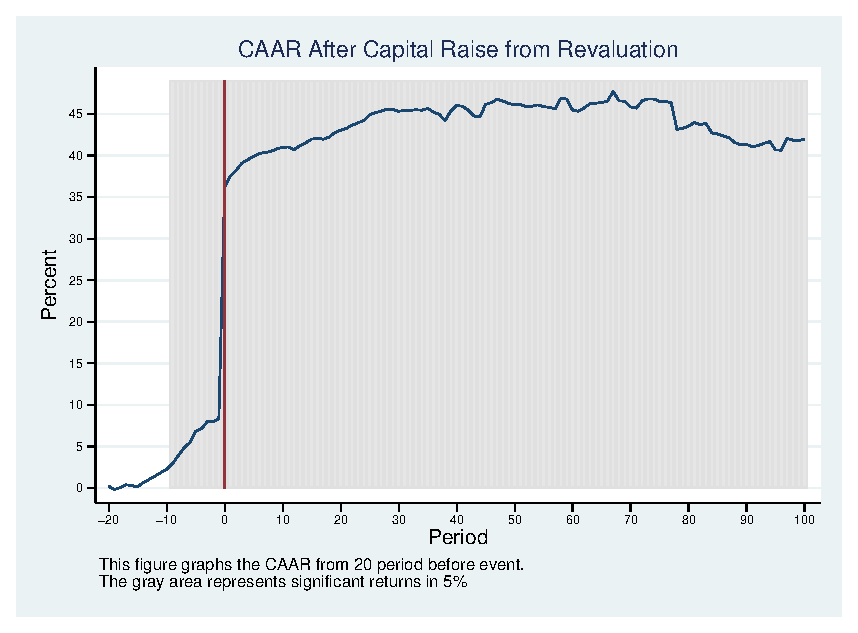
\includegraphics[width=0.65\linewidth]{AbReturnRevalution_WithoutAlpha}
\label{fig:abreturnrevalution3}
\end{figure}

\hfill\hyperlink{abreturnrevalution}{\beamerbutton{CAPM}}
\end{frame}


\begin{frame}{Abnormal Return}{Abnormal return of raised capital from Reserves}
\label{abreturnsavingWithoutAlpha}
\begin{figure}
\centering
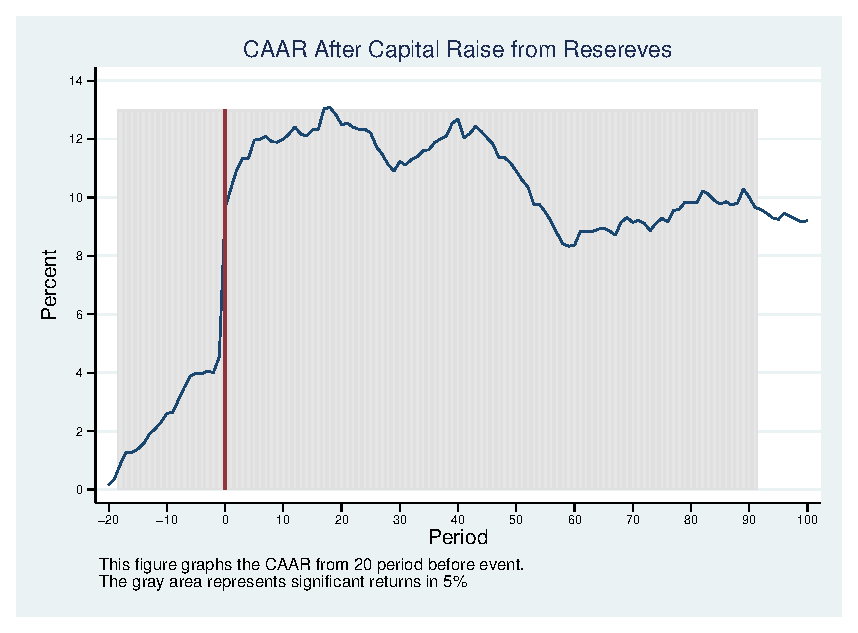
\includegraphics[width=0.65\linewidth]{AbReturnSaving_WithoutAlpha}
\label{fig:abreturnsaving3}
\end{figure}

\hfill\hyperlink{abreturnsaving}{\beamerbutton{CAPM}}
\end{frame}


\begin{frame}{Abnormal Return}{Abnormal return of raised capital from Cash}
\label{abreturncashWithoutAlpha}
\begin{figure}
\centering
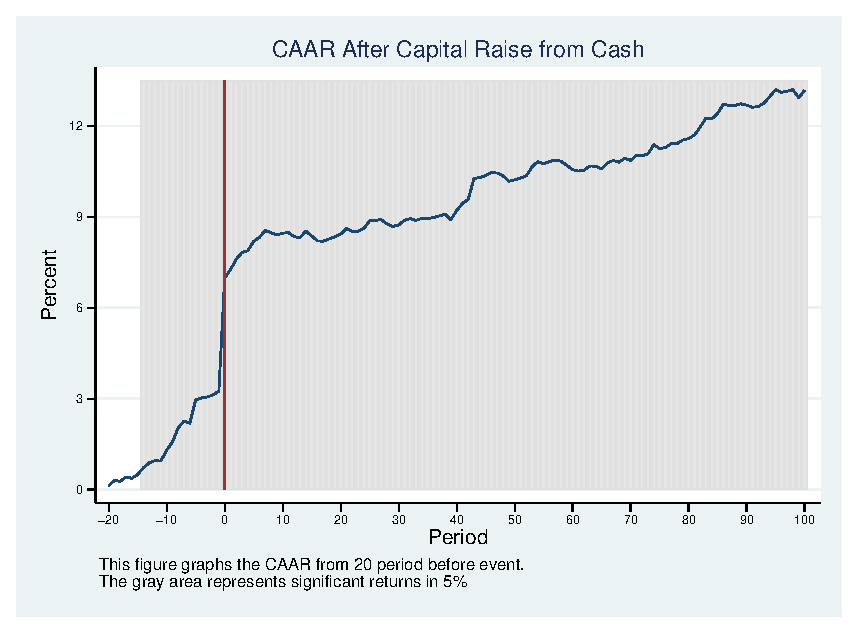
\includegraphics[width=0.65\linewidth]{AbReturnCash_WithoutAlpha}
\label{fig:abreturncash3}
\end{figure}
\hfill\hyperlink{abreturncash}{\beamerbutton{CAPM}}
\end{frame}


\begin{frame}{Abnormal Return}{Abnormal return of raised capital from Cash \& Reserves}
\label{abreturnhybridWithoutAlpha}
\begin{figure}
\centering
\includegraphics[width=0.65\linewidth]{AbReturnHybrid_WithoutAlpha}
\label{fig:abreturnhybrid3}
\end{figure}
\hfill\hyperlink{abreturnhybrid}{\beamerbutton{CAPM}}
\end{frame}



\section{Appendix II : Market}
\begin{frame}{Abnormal Return}
\label{abreturnMarket}
\begin{figure}
\centering
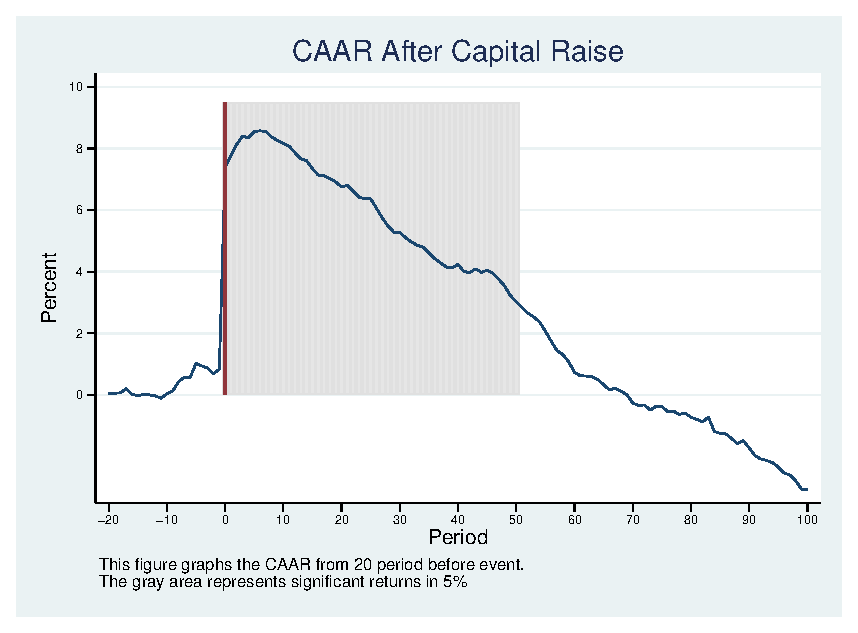
\includegraphics[width=0.7\linewidth]{AbReturn_Market.eps}
\label{fig:abreturn4}
\end{figure}
\hfill\hyperlink{abreturn}{\beamerbutton{CAPM}}
\end{frame}

\begin{frame}{Abnormal Return}{Abnormal return of raised capital from Revaluation}
\label{abreturnrevalutionMarket}
\begin{figure}
\centering
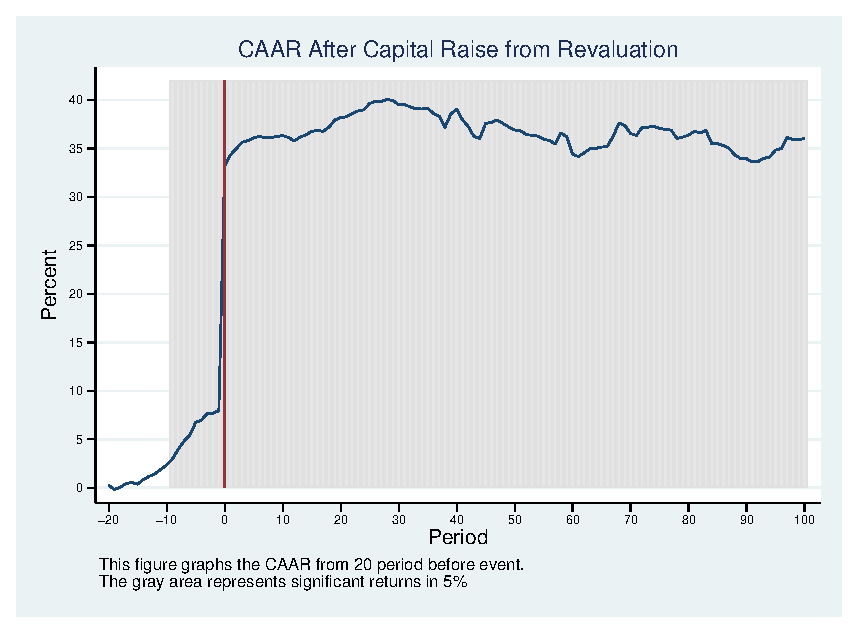
\includegraphics[width=0.65\linewidth]{AbReturnRevalution_Market}
\label{fig:abreturnrevalution4}
\end{figure}

\hfill\hyperlink{abreturnrevalution}{\beamerbutton{CAPM}}
\end{frame}


\begin{frame}{Abnormal Return}{Abnormal return of raised capital from Reserves}
\label{abreturnsavingMarket}
\begin{figure}
\centering
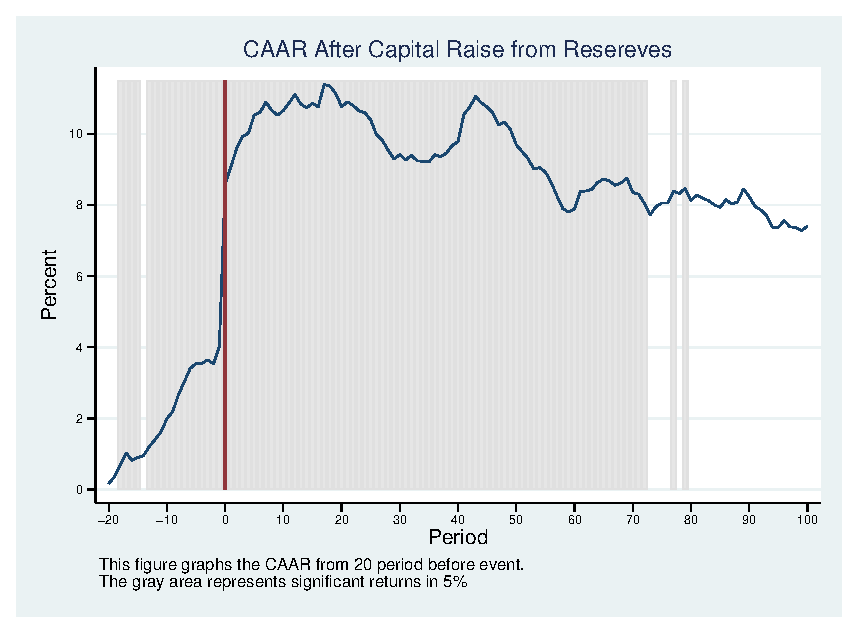
\includegraphics[width=0.65\linewidth]{AbReturnSaving_Market}
\label{fig:abreturnsaving4}
\end{figure}

\hfill\hyperlink{abreturnsaving}{\beamerbutton{CAPM}}
\end{frame}


\begin{frame}{Abnormal Return}{Abnormal return of raised capital from Cash}
\label{abreturncashMarket}
\begin{figure}
\centering
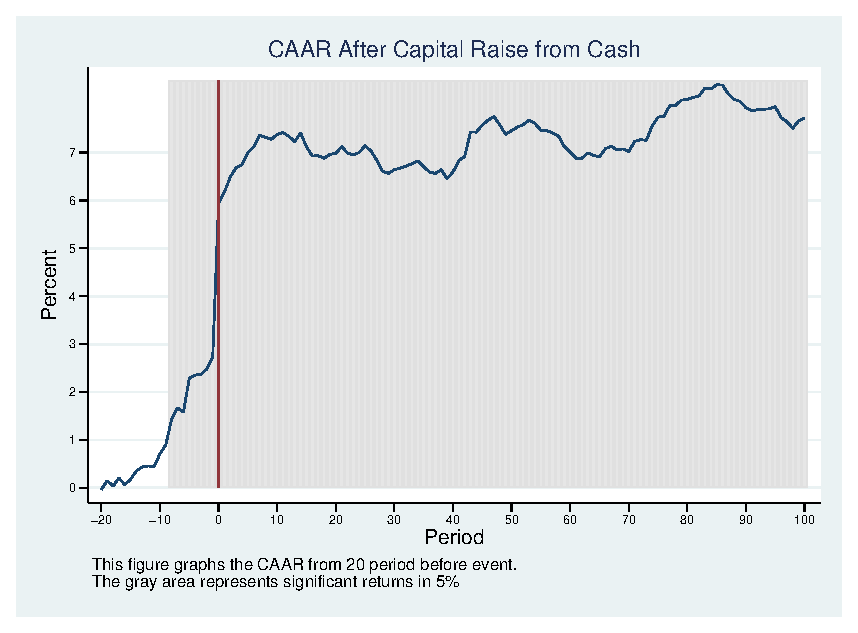
\includegraphics[width=0.65\linewidth]{AbReturnCash_Market}
\label{fig:abreturncash4}
\end{figure}
\hfill\hyperlink{abreturncash}{\beamerbutton{CAPM}}
\end{frame}


\begin{frame}{Abnormal Return}{Abnormal return of raised capital from Cash \& Reserves}
\label{abreturnhybridMarket}
\begin{figure}
\centering
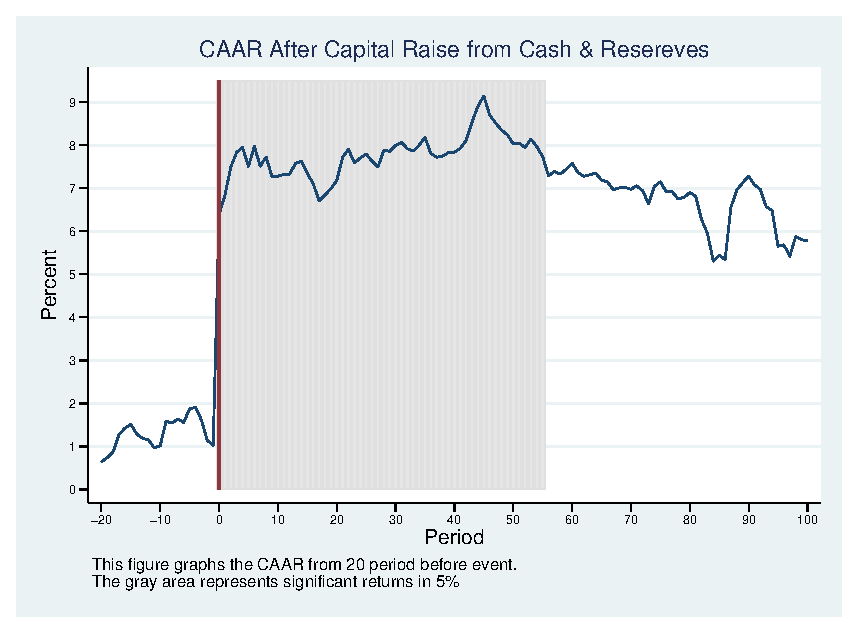
\includegraphics[width=0.65\linewidth]{AbReturnHybrid_Market}
\label{fig:abreturnhybrid4}
\end{figure}
\hfill\hyperlink{abreturnhybrid}{\beamerbutton{CAPM}}
\end{frame}




\section{Appendix II : Amihud}

\begin{frame}{Amihud}{Amihud of capital raise}
\begin{figure}
\centering
\includegraphics[width=0.7\linewidth]{Amihud}
\label{fig:amihud}
\end{figure}
\end{frame}



\begin{frame}{Amihud}{Amihud of raised capital from Revaluation}
\begin{figure}
\centering
\includegraphics[width=0.7\linewidth]{Amihud_Revaluation}
\label{fig:amihudrevaluation}
\end{figure}
\end{frame}

\begin{frame}{Amihud}{Amihud of raised capital that it's not from Revaluation}
\begin{figure}
\centering
\includegraphics[width=0.7\linewidth]{Amihud_NoRevaluation}
\label{fig:amihudnorevaluation}
\end{figure}
\end{frame}





\end{document}